\documentclass{report}

%%%%%%%%%%%%%%%%%%%%%%%%%%%%%%%%%
% PACKAGE IMPORTS
%%%%%%%%%%%%%%%%%%%%%%%%%%%%%%%%%


\usepackage[tmargin=2cm,rmargin=1in,lmargin=1in,margin=0.85in,bmargin=2cm,footskip=.2in]{geometry}
\usepackage{amsmath,amsfonts,amsthm,amssymb,mathtools}
\usepackage[varbb]{newpxmath}
\usepackage{xfrac}
\usepackage[makeroom]{cancel}
\usepackage{mathtools}
\usepackage{bookmark}
\usepackage{enumitem}
\usepackage{hyperref,theoremref}
\hypersetup{
	pdftitle={Assignment},
	colorlinks=true, linkcolor=doc!90,
	bookmarksnumbered=true,
	bookmarksopen=true
}
\usepackage[most,many,breakable]{tcolorbox}
\usepackage{xcolor}
\usepackage{varwidth}
\usepackage{varwidth}
\usepackage{etoolbox}
%\usepackage{authblk}
\usepackage{nameref}
\usepackage{multicol,array}
\usepackage{tikz-cd}
\usepackage[ruled,vlined,linesnumbered]{algorithm2e}
\usepackage{comment} % enables the use of multi-line comments (\ifx \fi) 
\usepackage{import}
\usepackage{xifthen}
\usepackage{pdfpages}
\usepackage{transparent}

\newcommand\mycommfont[1]{\footnotesize\ttfamily\textcolor{blue}{#1}}
\SetCommentSty{mycommfont}
\newcommand{\incfig}[1]{%
    \def\svgwidth{\columnwidth}
    \import{./figures/}{#1.pdf_tex}
}

\usepackage{tikzsymbols}
\renewcommand\qedsymbol{$\Laughey$}


%\usepackage{import}
%\usepackage{xifthen}
%\usepackage{pdfpages}
%\usepackage{transparent}


%%%%%%%%%%%%%%%%%%%%%%%%%%%%%%
% SELF MADE COLORS
%%%%%%%%%%%%%%%%%%%%%%%%%%%%%%



\definecolor{myg}{RGB}{56, 140, 70}
\definecolor{myb}{RGB}{45, 111, 177}
\definecolor{myr}{RGB}{199, 68, 64}
\definecolor{mytheorembg}{HTML}{F2F2F9}
\definecolor{mytheoremfr}{HTML}{00007B}
\definecolor{mylenmabg}{HTML}{FFFAF8}
\definecolor{mylenmafr}{HTML}{983b0f}
\definecolor{mypropbg}{HTML}{f2fbfc}
\definecolor{mypropfr}{HTML}{191971}
\definecolor{myexamplebg}{HTML}{F2FBF8}
\definecolor{myexamplefr}{HTML}{88D6D1}
\definecolor{myexampleti}{HTML}{2A7F7F}
\definecolor{mydefinitbg}{HTML}{E5E5FF}
\definecolor{mydefinitfr}{HTML}{3F3FA3}
\definecolor{notesgreen}{RGB}{0,162,0}
\definecolor{myp}{RGB}{197, 92, 212}
\definecolor{mygr}{HTML}{2C3338}
\definecolor{myred}{RGB}{127,0,0}
\definecolor{myyellow}{RGB}{169,121,69}
\definecolor{myexercisebg}{HTML}{F2FBF8}
\definecolor{myexercisefg}{HTML}{88D6D1}


%%%%%%%%%%%%%%%%%%%%%%%%%%%%
% TCOLORBOX SETUPS
%%%%%%%%%%%%%%%%%%%%%%%%%%%%

\setlength{\parindent}{1cm}
%================================
% THEOREM BOX
%================================

\tcbuselibrary{theorems,skins,hooks}
\newtcbtheorem[number within=section]{Theorem}{Theorem}
{%
	enhanced,
	breakable,
	colback = mytheorembg,
	frame hidden,
	boxrule = 0sp,
	borderline west = {2pt}{0pt}{mytheoremfr},
	sharp corners,
	detach title,
	before upper = \tcbtitle\par\smallskip,
	coltitle = mytheoremfr,
	fonttitle = \bfseries\sffamily,
	description font = \mdseries,
	separator sign none,
	segmentation style={solid, mytheoremfr},
}
{th}

\tcbuselibrary{theorems,skins,hooks}
\newtcbtheorem[number within=chapter]{theorem}{Theorem}
{%
	enhanced,
	breakable,
	colback = mytheorembg,
	frame hidden,
	boxrule = 0sp,
	borderline west = {2pt}{0pt}{mytheoremfr},
	sharp corners,
	detach title,
	before upper = \tcbtitle\par\smallskip,
	coltitle = mytheoremfr,
	fonttitle = \bfseries\sffamily,
	description font = \mdseries,
	separator sign none,
	segmentation style={solid, mytheoremfr},
}
{th}


\tcbuselibrary{theorems,skins,hooks}
\newtcolorbox{Theoremcon}
{%
	enhanced
	,breakable
	,colback = mytheorembg
	,frame hidden
	,boxrule = 0sp
	,borderline west = {2pt}{0pt}{mytheoremfr}
	,sharp corners
	,description font = \mdseries
	,separator sign none
}

%================================
% Corollary
%================================
\tcbuselibrary{theorems,skins,hooks}
\newtcbtheorem[number within=section]{Corollary}{Corollary}
{%
	enhanced
	,breakable
	,colback = myp!10
	,frame hidden
	,boxrule = 0sp
	,borderline west = {2pt}{0pt}{myp!85!black}
	,sharp corners
	,detach title
	,before upper = \tcbtitle\par\smallskip
	,coltitle = myp!85!black
	,fonttitle = \bfseries\sffamily
	,description font = \mdseries
	,separator sign none
	,segmentation style={solid, myp!85!black}
}
{th}
\tcbuselibrary{theorems,skins,hooks}
\newtcbtheorem[number within=chapter]{corollary}{Corollary}
{%
	enhanced
	,breakable
	,colback = myp!10
	,frame hidden
	,boxrule = 0sp
	,borderline west = {2pt}{0pt}{myp!85!black}
	,sharp corners
	,detach title
	,before upper = \tcbtitle\par\smallskip
	,coltitle = myp!85!black
	,fonttitle = \bfseries\sffamily
	,description font = \mdseries
	,separator sign none
	,segmentation style={solid, myp!85!black}
}
{th}


%================================
% LENMA
%================================

\tcbuselibrary{theorems,skins,hooks}
\newtcbtheorem[number within=section]{Lenma}{Lenma}
{%
	enhanced,
	breakable,
	colback = mylenmabg,
	frame hidden,
	boxrule = 0sp,
	borderline west = {2pt}{0pt}{mylenmafr},
	sharp corners,
	detach title,
	before upper = \tcbtitle\par\smallskip,
	coltitle = mylenmafr,
	fonttitle = \bfseries\sffamily,
	description font = \mdseries,
	separator sign none,
	segmentation style={solid, mylenmafr},
}
{th}

\tcbuselibrary{theorems,skins,hooks}
\newtcbtheorem[number within=chapter]{lenma}{Lenma}
{%
	enhanced,
	breakable,
	colback = mylenmabg,
	frame hidden,
	boxrule = 0sp,
	borderline west = {2pt}{0pt}{mylenmafr},
	sharp corners,
	detach title,
	before upper = \tcbtitle\par\smallskip,
	coltitle = mylenmafr,
	fonttitle = \bfseries\sffamily,
	description font = \mdseries,
	separator sign none,
	segmentation style={solid, mylenmafr},
}
{th}


%================================
% PROPOSITION
%================================

\tcbuselibrary{theorems,skins,hooks}
\newtcbtheorem[number within=section]{Prop}{Proposition}
{%
	enhanced,
	breakable,
	colback = mypropbg,
	frame hidden,
	boxrule = 0sp,
	borderline west = {2pt}{0pt}{mypropfr},
	sharp corners,
	detach title,
	before upper = \tcbtitle\par\smallskip,
	coltitle = mypropfr,
	fonttitle = \bfseries\sffamily,
	description font = \mdseries,
	separator sign none,
	segmentation style={solid, mypropfr},
}
{th}

\tcbuselibrary{theorems,skins,hooks}
\newtcbtheorem[number within=chapter]{prop}{Proposition}
{%
	enhanced,
	breakable,
	colback = mypropbg,
	frame hidden,
	boxrule = 0sp,
	borderline west = {2pt}{0pt}{mypropfr},
	sharp corners,
	detach title,
	before upper = \tcbtitle\par\smallskip,
	coltitle = mypropfr,
	fonttitle = \bfseries\sffamily,
	description font = \mdseries,
	separator sign none,
	segmentation style={solid, mypropfr},
}
{th}


%================================
% CLAIM
%================================

\tcbuselibrary{theorems,skins,hooks}
\newtcbtheorem[number within=section]{claim}{Claim}
{%
	enhanced
	,breakable
	,colback = myg!10
	,frame hidden
	,boxrule = 0sp
	,borderline west = {2pt}{0pt}{myg}
	,sharp corners
	,detach title
	,before upper = \tcbtitle\par\smallskip
	,coltitle = myg!85!black
	,fonttitle = \bfseries\sffamily
	,description font = \mdseries
	,separator sign none
	,segmentation style={solid, myg!85!black}
}
{th}



%================================
% Exercise
%================================

\tcbuselibrary{theorems,skins,hooks}
\newtcbtheorem[number within=section]{Exercise}{Exercise}
{%
	enhanced,
	breakable,
	colback = myexercisebg,
	frame hidden,
	boxrule = 0sp,
	borderline west = {2pt}{0pt}{myexercisefg},
	sharp corners,
	detach title,
	before upper = \tcbtitle\par\smallskip,
	coltitle = myexercisefg,
	fonttitle = \bfseries\sffamily,
	description font = \mdseries,
	separator sign none,
	segmentation style={solid, myexercisefg},
}
{th}

\tcbuselibrary{theorems,skins,hooks}
\newtcbtheorem[number within=chapter]{exercise}{Exercise}
{%
	enhanced,
	breakable,
	colback = myexercisebg,
	frame hidden,
	boxrule = 0sp,
	borderline west = {2pt}{0pt}{myexercisefg},
	sharp corners,
	detach title,
	before upper = \tcbtitle\par\smallskip,
	coltitle = myexercisefg,
	fonttitle = \bfseries\sffamily,
	description font = \mdseries,
	separator sign none,
	segmentation style={solid, myexercisefg},
}
{th}

%================================
% EXAMPLE BOX
%================================

\newtcbtheorem[number within=section]{Example}{Example}
{%
	colback = myexamplebg
	,breakable
	,colframe = myexamplefr
	,coltitle = myexampleti
	,boxrule = 1pt
	,sharp corners
	,detach title
	,before upper=\tcbtitle\par\smallskip
	,fonttitle = \bfseries
	,description font = \mdseries
	,separator sign none
	,description delimiters parenthesis
}
{ex}

\newtcbtheorem[number within=chapter]{example}{Example}
{%
	colback = myexamplebg
	,breakable
	,colframe = myexamplefr
	,coltitle = myexampleti
	,boxrule = 1pt
	,sharp corners
	,detach title
	,before upper=\tcbtitle\par\smallskip
	,fonttitle = \bfseries
	,description font = \mdseries
	,separator sign none
	,description delimiters parenthesis
}
{ex}

%================================
% DEFINITION BOX
%================================

\newtcbtheorem[number within=section]{Definition}{Definition}{enhanced,
	before skip=2mm,after skip=2mm, colback=red!5,colframe=red!80!black,boxrule=0.5mm,
	attach boxed title to top left={xshift=1cm,yshift*=1mm-\tcboxedtitleheight}, varwidth boxed title*=-3cm,
	boxed title style={frame code={
					\path[fill=tcbcolback]
					([yshift=-1mm,xshift=-1mm]frame.north west)
					arc[start angle=0,end angle=180,radius=1mm]
					([yshift=-1mm,xshift=1mm]frame.north east)
					arc[start angle=180,end angle=0,radius=1mm];
					\path[left color=tcbcolback!60!black,right color=tcbcolback!60!black,
						middle color=tcbcolback!80!black]
					([xshift=-2mm]frame.north west) -- ([xshift=2mm]frame.north east)
					[rounded corners=1mm]-- ([xshift=1mm,yshift=-1mm]frame.north east)
					-- (frame.south east) -- (frame.south west)
					-- ([xshift=-1mm,yshift=-1mm]frame.north west)
					[sharp corners]-- cycle;
				},interior engine=empty,
		},
	fonttitle=\bfseries,
	title={#2},#1}{def}
\newtcbtheorem[number within=chapter]{definition}{Definition}{enhanced,
	before skip=2mm,after skip=2mm, colback=red!5,colframe=red!80!black,boxrule=0.5mm,
	attach boxed title to top left={xshift=1cm,yshift*=1mm-\tcboxedtitleheight}, varwidth boxed title*=-3cm,
	boxed title style={frame code={
					\path[fill=tcbcolback]
					([yshift=-1mm,xshift=-1mm]frame.north west)
					arc[start angle=0,end angle=180,radius=1mm]
					([yshift=-1mm,xshift=1mm]frame.north east)
					arc[start angle=180,end angle=0,radius=1mm];
					\path[left color=tcbcolback!60!black,right color=tcbcolback!60!black,
						middle color=tcbcolback!80!black]
					([xshift=-2mm]frame.north west) -- ([xshift=2mm]frame.north east)
					[rounded corners=1mm]-- ([xshift=1mm,yshift=-1mm]frame.north east)
					-- (frame.south east) -- (frame.south west)
					-- ([xshift=-1mm,yshift=-1mm]frame.north west)
					[sharp corners]-- cycle;
				},interior engine=empty,
		},
	fonttitle=\bfseries,
	title={#2},#1}{def}



%================================
% Solution BOX
%================================

\makeatletter
\newtcbtheorem{question}{Question}{enhanced,
	breakable,
	colback=white,
	colframe=myb!80!black,
	attach boxed title to top left={yshift*=-\tcboxedtitleheight},
	fonttitle=\bfseries,
	title={#2},
	boxed title size=title,
	boxed title style={%
			sharp corners,
			rounded corners=northwest,
			colback=tcbcolframe,
			boxrule=0pt,
		},
	underlay boxed title={%
			\path[fill=tcbcolframe] (title.south west)--(title.south east)
			to[out=0, in=180] ([xshift=5mm]title.east)--
			(title.center-|frame.east)
			[rounded corners=\kvtcb@arc] |-
			(frame.north) -| cycle;
		},
	#1
}{def}
\makeatother

%================================
% SOLUTION BOX
%================================

\makeatletter
\newtcolorbox{solution}{enhanced,
	breakable,
	colback=white,
	colframe=myg!80!black,
	attach boxed title to top left={yshift*=-\tcboxedtitleheight},
	title=Solution,
	boxed title size=title,
	boxed title style={%
			sharp corners,
			rounded corners=northwest,
			colback=tcbcolframe,
			boxrule=0pt,
		},
	underlay boxed title={%
			\path[fill=tcbcolframe] (title.south west)--(title.south east)
			to[out=0, in=180] ([xshift=5mm]title.east)--
			(title.center-|frame.east)
			[rounded corners=\kvtcb@arc] |-
			(frame.north) -| cycle;
		},
}
\makeatother

%================================
% Question BOX
%================================

\makeatletter
\newtcbtheorem{qstion}{Question}{enhanced,
	breakable,
	colback=white,
	colframe=mygr,
	attach boxed title to top left={yshift*=-\tcboxedtitleheight},
	fonttitle=\bfseries,
	title={#2},
	boxed title size=title,
	boxed title style={%
			sharp corners,
			rounded corners=northwest,
			colback=tcbcolframe,
			boxrule=0pt,
		},
	underlay boxed title={%
			\path[fill=tcbcolframe] (title.south west)--(title.south east)
			to[out=0, in=180] ([xshift=5mm]title.east)--
			(title.center-|frame.east)
			[rounded corners=\kvtcb@arc] |-
			(frame.north) -| cycle;
		},
	#1
}{def}
\makeatother

\newtcbtheorem[number within=chapter]{wconc}{Wrong Concept}{
	breakable,
	enhanced,
	colback=white,
	colframe=myr,
	arc=0pt,
	outer arc=0pt,
	fonttitle=\bfseries\sffamily\large,
	colbacktitle=myr,
	attach boxed title to top left={},
	boxed title style={
			enhanced,
			skin=enhancedfirst jigsaw,
			arc=3pt,
			bottom=0pt,
			interior style={fill=myr}
		},
	#1
}{def}



%================================
% NOTE BOX
%================================

\usetikzlibrary{arrows,calc,shadows.blur}
\tcbuselibrary{skins}
\newtcolorbox{note}[1][]{%
	enhanced jigsaw,
	colback=gray!20!white,%
	colframe=gray!80!black,
	size=small,
	boxrule=1pt,
	title=\textbf{Note:-},
	halign title=flush center,
	coltitle=black,
	breakable,
	drop shadow=black!50!white,
	attach boxed title to top left={xshift=1cm,yshift=-\tcboxedtitleheight/2,yshifttext=-\tcboxedtitleheight/2},
	minipage boxed title=1.5cm,
	boxed title style={%
			colback=white,
			size=fbox,
			boxrule=1pt,
			boxsep=2pt,
			underlay={%
					\coordinate (dotA) at ($(interior.west) + (-0.5pt,0)$);
					\coordinate (dotB) at ($(interior.east) + (0.5pt,0)$);
					\begin{scope}
						\clip (interior.north west) rectangle ([xshift=3ex]interior.east);
						\filldraw [white, blur shadow={shadow opacity=60, shadow yshift=-.75ex}, rounded corners=2pt] (interior.north west) rectangle (interior.south east);
					\end{scope}
					\begin{scope}[gray!80!black]
						\fill (dotA) circle (2pt);
						\fill (dotB) circle (2pt);
					\end{scope}
				},
		},
	#1,
}

%%%%%%%%%%%%%%%%%%%%%%%%%%%%%%
% SELF MADE COMMANDS
%%%%%%%%%%%%%%%%%%%%%%%%%%%%%%


\newcommand{\thm}[2]{\begin{Theorem}{#1}{}#2\end{Theorem}}
\newcommand{\cor}[2]{\begin{Corollary}{#1}{}#2\end{Corollary}}
\newcommand{\mlenma}[2]{\begin{Lenma}{#1}{}#2\end{Lenma}}
\newcommand{\mprop}[2]{\begin{Prop}{#1}{}#2\end{Prop}}
\newcommand{\clm}[3]{\begin{claim}{#1}{#2}#3\end{claim}}
\newcommand{\wc}[2]{\begin{wconc}{#1}{}\setlength{\parindent}{1cm}#2\end{wconc}}
\newcommand{\thmcon}[1]{\begin{Theoremcon}{#1}\end{Theoremcon}}
\newcommand{\ex}[2]{\begin{Example}{#1}{}#2\end{Example}}
\newcommand{\dfn}[2]{\begin{Definition}[colbacktitle=red!75!black]{#1}{}#2\end{Definition}}
\newcommand{\dfnc}[2]{\begin{definition}[colbacktitle=red!75!black]{#1}{}#2\end{definition}}
\newcommand{\qs}[2]{\begin{question}{#1}{}#2\end{question}}
\newcommand{\pf}[2]{\begin{myproof}[#1]#2\end{myproof}}
\newcommand{\nt}[1]{\begin{note}#1\end{note}}

\newcommand*\circled[1]{\tikz[baseline=(char.base)]{
		\node[shape=circle,draw,inner sep=1pt] (char) {#1};}}
\newcommand\getcurrentref[1]{%
	\ifnumequal{\value{#1}}{0}
	{??}
	{\the\value{#1}}%
}
\newcommand{\getCurrentSectionNumber}{\getcurrentref{section}}
\newenvironment{myproof}[1][\proofname]{%
	\proof[\bfseries #1: ]%
}{\endproof}

\newcommand{\mclm}[2]{\begin{myclaim}[#1]#2\end{myclaim}}
\newenvironment{myclaim}[1][\claimname]{\proof[\bfseries #1: ]}{}

\newcounter{mylabelcounter}

\makeatletter
\newcommand{\setword}[2]{%
	\phantomsection
	#1\def\@currentlabel{\unexpanded{#1}}\label{#2}%
}
\makeatother




\tikzset{
	symbol/.style={
			draw=none,
			every to/.append style={
					edge node={node [sloped, allow upside down, auto=false]{$#1$}}}
		}
}


% deliminators
\DeclarePairedDelimiter{\abs}{\lvert}{\rvert}
\DeclarePairedDelimiter{\norm}{\lVert}{\rVert}

\DeclarePairedDelimiter{\ceil}{\lceil}{\rceil}
\DeclarePairedDelimiter{\floor}{\lfloor}{\rfloor}
\DeclarePairedDelimiter{\round}{\lfloor}{\rceil}

\newsavebox\diffdbox
\newcommand{\slantedromand}{{\mathpalette\makesl{d}}}
\newcommand{\makesl}[2]{%
\begingroup
\sbox{\diffdbox}{$\mathsurround=0pt#1\mathrm{#2}$}%
\pdfsave
\pdfsetmatrix{1 0 0.2 1}%
\rlap{\usebox{\diffdbox}}%
\pdfrestore
\hskip\wd\diffdbox
\endgroup
}
\newcommand{\dd}[1][]{\ensuremath{\mathop{}\!\ifstrempty{#1}{%
\slantedromand\@ifnextchar^{\hspace{0.2ex}}{\hspace{0.1ex}}}%
{\slantedromand\hspace{0.2ex}^{#1}}}}
\ProvideDocumentCommand\dv{o m g}{%
  \ensuremath{%
    \IfValueTF{#3}{%
      \IfNoValueTF{#1}{%
        \frac{\dd #2}{\dd #3}%
      }{%
        \frac{\dd^{#1} #2}{\dd #3^{#1}}%
      }%
    }{%
      \IfNoValueTF{#1}{%
        \frac{\dd}{\dd #2}%
      }{%
        \frac{\dd^{#1}}{\dd #2^{#1}}%
      }%
    }%
  }%
}
\providecommand*{\pdv}[3][]{\frac{\partial^{#1}#2}{\partial#3^{#1}}}
%  - others
\DeclareMathOperator{\Lap}{\mathcal{L}}
\DeclareMathOperator{\Var}{Var} % varience
\DeclareMathOperator{\Cov}{Cov} % covarience
\DeclareMathOperator{\E}{E} % expected

% Since the amsthm package isn't loaded

% I prefer the slanted \leq
\let\oldleq\leq % save them in case they're every wanted
\let\oldgeq\geq
\renewcommand{\leq}{\leqslant}
\renewcommand{\geq}{\geqslant}

% % redefine matrix env to allow for alignment, use r as default
% \renewcommand*\env@matrix[1][r]{\hskip -\arraycolsep
%     \let\@ifnextchar\new@ifnextchar
%     \array{*\c@MaxMatrixCols #1}}


%\usepackage{framed}
%\usepackage{titletoc}
%\usepackage{etoolbox}
%\usepackage{lmodern}


%\patchcmd{\tableofcontents}{\contentsname}{\sffamily\contentsname}{}{}

%\renewenvironment{leftbar}
%{\def\FrameCommand{\hspace{6em}%
%		{\color{myyellow}\vrule width 2pt depth 6pt}\hspace{1em}}%
%	\MakeFramed{\parshape 1 0cm \dimexpr\textwidth-6em\relax\FrameRestore}\vskip2pt%
%}
%{\endMakeFramed}

%\titlecontents{chapter}
%[0em]{\vspace*{2\baselineskip}}
%{\parbox{4.5em}{%
%		\hfill\Huge\sffamily\bfseries\color{myred}\thecontentspage}%
%	\vspace*{-2.3\baselineskip}\leftbar\textsc{\small\chaptername~\thecontentslabel}\\\sffamily}
%{}{\endleftbar}
%\titlecontents{section}
%[8.4em]
%{\sffamily\contentslabel{3em}}{}{}
%{\hspace{0.5em}\nobreak\itshape\color{myred}\contentspage}
%\titlecontents{subsection}
%[8.4em]
%{\sffamily\contentslabel{3em}}{}{}  
%{\hspace{0.5em}\nobreak\itshape\color{myred}\contentspage}



%%%%%%%%%%%%%%%%%%%%%%%%%%%%%%%%%%%%%%%%%%%
% TABLE OF CONTENTS
%%%%%%%%%%%%%%%%%%%%%%%%%%%%%%%%%%%%%%%%%%%

\usepackage{tikz}
\definecolor{doc}{RGB}{0,60,110}
\usepackage{titletoc}
\contentsmargin{0cm}
\titlecontents{chapter}[3.7pc]
{\addvspace{30pt}%
	\begin{tikzpicture}[remember picture, overlay]%
		\draw[fill=doc!60,draw=doc!60] (-7,-.1) rectangle (-0.9,.5);%
		\pgftext[left,x=-3.5cm,y=0.2cm]{\color{white}\Large\sc\bfseries Chapter\ \thecontentslabel};%
	\end{tikzpicture}\color{doc!60}\large\sc\bfseries}%
{}
{}
{\;\titlerule\;\large\sc\bfseries Page \thecontentspage
	\begin{tikzpicture}[remember picture, overlay]
		\draw[fill=doc!60,draw=doc!60] (2pt,0) rectangle (4,0.1pt);
	\end{tikzpicture}}%
\titlecontents{section}[3.7pc]
{\addvspace{2pt}}
{\contentslabel[\thecontentslabel]{2pc}}
{}
{\hfill\small \thecontentspage}
[]
\titlecontents*{subsection}[3.7pc]
{\addvspace{-1pt}\small}
{}
{}
{\ --- \small\thecontentspage}
[ \textbullet\ ][]

\makeatletter
\renewcommand{\tableofcontents}{%
	\chapter*{%
	  \vspace*{-20\p@}%
	  \begin{tikzpicture}[remember picture, overlay]%
		  \pgftext[right,x=15cm,y=0.2cm]{\color{doc!60}\Huge\sc\bfseries \contentsname};%
		  \draw[fill=doc!60,draw=doc!60] (13,-.75) rectangle (20,1);%
		  \clip (13,-.75) rectangle (20,1);
		  \pgftext[right,x=15cm,y=0.2cm]{\color{white}\Huge\sc\bfseries \contentsname};%
	  \end{tikzpicture}}%
	\@starttoc{toc}}
\makeatother

%From M275 "Topology" at SJSU
\newcommand{\id}{\mathrm{id}}
\newcommand{\taking}[1]{\xrightarrow{#1}}
\newcommand{\inv}{^{-1}}

%From M170 "Introduction to Graph Theory" at SJSU
\DeclareMathOperator{\diam}{diam}
\DeclareMathOperator{\ord}{ord}
\newcommand{\defeq}{\overset{\mathrm{def}}{=}}

%From the USAMO .tex files
\newcommand{\ts}{\textsuperscript}
\newcommand{\dg}{^\circ}
\newcommand{\ii}{\item}

% % From Math 55 and Math 145 at Harvard
% \newenvironment{subproof}[1][Proof]{%
% \begin{proof}[#1] \renewcommand{\qedsymbol}{$\blacksquare$}}%
% {\end{proof}}

\newcommand{\liff}{\leftrightarrow}
\newcommand{\lthen}{\rightarrow}
\newcommand{\opname}{\operatorname}
\newcommand{\surjto}{\twoheadrightarrow}
\newcommand{\injto}{\hookrightarrow}
\newcommand{\On}{\mathrm{On}} % ordinals
\DeclareMathOperator{\img}{im} % Image
\DeclareMathOperator{\Img}{Im} % Image
\DeclareMathOperator{\coker}{coker} % Cokernel
\DeclareMathOperator{\Coker}{Coker} % Cokernel
\DeclareMathOperator{\Ker}{Ker} % Kernel
\DeclareMathOperator{\rank}{rank}
\DeclareMathOperator{\Spec}{Spec} % spectrum
\DeclareMathOperator{\Tr}{Tr} % trace
\DeclareMathOperator{\pr}{pr} % projection
\DeclareMathOperator{\ext}{ext} % extension
\DeclareMathOperator{\pred}{pred} % predecessor
\DeclareMathOperator{\dom}{dom} % domain
\DeclareMathOperator{\ran}{ran} % range
\DeclareMathOperator{\Hom}{Hom} % homomorphism
\DeclareMathOperator{\Mor}{Mor} % morphisms
\DeclareMathOperator{\End}{End} % endomorphism

\def\shrug{\texttt{\raisebox{0.75em}{\char`\_}\char`\\\char`\_\kern-0.5ex(\kern-0.25ex\raisebox{0.25ex}{\rotatebox{45}{\raisebox{-.75ex}"\kern-1.5ex\rotatebox{-90})}}\kern-0.5ex)\kern-0.5ex\char`\_/\raisebox{0.75em}{\char`\_}}} 

\newcommand{\eps}{\epsilon}
\newcommand{\veps}{\varepsilon}
\newcommand{\ol}{\overline}
\newcommand{\ul}{\underline}
\newcommand{\wt}{\widetilde}
\newcommand{\wh}{\widehat}
\newcommand{\vocab}[1]{\textbf{\color{blue} #1}}
\providecommand{\half}{\frac{1}{2}}
\newcommand{\dang}{\measuredangle} %% Directed angle
\newcommand{\ray}[1]{\overrightarrow{#1}}
\newcommand{\seg}[1]{\overline{#1}}
\newcommand{\arc}[1]{\wideparen{#1}}
\DeclareMathOperator{\cis}{cis}
\DeclareMathOperator*{\lcm}{lcm}
\DeclareMathOperator*{\argmin}{arg min}
\DeclareMathOperator*{\argmax}{arg max}
\newcommand{\cycsum}{\sum_{\mathrm{cyc}}}
\newcommand{\symsum}{\sum_{\mathrm{sym}}}
\newcommand{\cycprod}{\prod_{\mathrm{cyc}}}
\newcommand{\symprod}{\prod_{\mathrm{sym}}}
\newcommand{\Qed}{\begin{flushright}\qed\end{flushright}}
\newcommand{\parinn}{\setlength{\parindent}{1cm}}
\newcommand{\parinf}{\setlength{\parindent}{0cm}}
% \newcommand{\norm}{\|\cdot\|}
\newcommand{\inorm}{\norm_{\infty}}
\newcommand{\opensets}{\{V_{\alpha}\}_{\alpha\in I}}
\newcommand{\oset}{V_{\alpha}}
\newcommand{\opset}[1]{V_{\alpha_{#1}}}
\newcommand{\lub}{\text{lub}}
\newcommand{\del}[2]{\frac{\partial #1}{\partial #2}}
\newcommand{\Del}[3]{\frac{\partial^{#1} #2}{\partial^{#1} #3}}
\newcommand{\deld}[2]{\dfrac{\partial #1}{\partial #2}}
\newcommand{\Deld}[3]{\dfrac{\partial^{#1} #2}{\partial^{#1} #3}}
\newcommand{\lm}{\lambda}
\newcommand{\uin}{\mathbin{\rotatebox[origin=c]{90}{$\in$}}}
\newcommand{\usubset}{\mathbin{\rotatebox[origin=c]{90}{$\subset$}}}
\newcommand{\lt}{\left}
\newcommand{\rt}{\right}
\newcommand{\bs}[1]{\boldsymbol{#1}}
\newcommand{\exs}{\exists}
\newcommand{\st}{\strut}
\newcommand{\dps}[1]{\displaystyle{#1}}

\newcommand{\sol}{\setlength{\parindent}{0cm}\textbf{\textit{Solution:}}\setlength{\parindent}{1cm} }
\newcommand{\solve}[1]{\setlength{\parindent}{0cm}\textbf{\textit{Solution: }}\setlength{\parindent}{1cm}#1 \Qed}
% Things Lie
\newcommand{\kb}{\mathfrak b}
\newcommand{\kg}{\mathfrak g}
\newcommand{\kh}{\mathfrak h}
\newcommand{\kn}{\mathfrak n}
\newcommand{\ku}{\mathfrak u}
\newcommand{\kz}{\mathfrak z}
\DeclareMathOperator{\Ext}{Ext} % Ext functor
\DeclareMathOperator{\Tor}{Tor} % Tor functor
\newcommand{\gl}{\opname{\mathfrak{gl}}} % frak gl group
\renewcommand{\sl}{\opname{\mathfrak{sl}}} % frak sl group chktex 6

% More script letters etc.
\newcommand{\SA}{\mathcal A}
\newcommand{\SB}{\mathcal B}
\newcommand{\SC}{\mathcal C}
\newcommand{\SF}{\mathcal F}
\newcommand{\SG}{\mathcal G}
\newcommand{\SH}{\mathcal H}
\newcommand{\OO}{\mathcal O}

\newcommand{\SCA}{\mathscr A}
\newcommand{\SCB}{\mathscr B}
\newcommand{\SCC}{\mathscr C}
\newcommand{\SCD}{\mathscr D}
\newcommand{\SCE}{\mathscr E}
\newcommand{\SCF}{\mathscr F}
\newcommand{\SCG}{\mathscr G}
\newcommand{\SCH}{\mathscr H}

% Mathfrak primes
\newcommand{\km}{\mathfrak m}
\newcommand{\kp}{\mathfrak p}
\newcommand{\kq}{\mathfrak q}

% number sets
\newcommand{\RR}[1][]{\ensuremath{\ifstrempty{#1}{\mathbb{R}}{\mathbb{R}^{#1}}}}
\newcommand{\NN}[1][]{\ensuremath{\ifstrempty{#1}{\mathbb{N}}{\mathbb{N}^{#1}}}}
\newcommand{\ZZ}[1][]{\ensuremath{\ifstrempty{#1}{\mathbb{Z}}{\mathbb{Z}^{#1}}}}
\newcommand{\QQ}[1][]{\ensuremath{\ifstrempty{#1}{\mathbb{Q}}{\mathbb{Q}^{#1}}}}
\newcommand{\CC}[1][]{\ensuremath{\ifstrempty{#1}{\mathbb{C}}{\mathbb{C}^{#1}}}}
\newcommand{\PP}[1][]{\ensuremath{\ifstrempty{#1}{\mathbb{P}}{\mathbb{P}^{#1}}}}
\newcommand{\HH}[1][]{\ensuremath{\ifstrempty{#1}{\mathbb{H}}{\mathbb{H}^{#1}}}}
\newcommand{\FF}[1][]{\ensuremath{\ifstrempty{#1}{\mathbb{F}}{\mathbb{F}^{#1}}}}
% expected value
\newcommand{\EE}{\ensuremath{\mathbb{E}}}
\newcommand{\charin}{\text{ char }}
\DeclareMathOperator{\sign}{sign}
\DeclareMathOperator{\Aut}{Aut}
\DeclareMathOperator{\Inn}{Inn}
\DeclareMathOperator{\Syl}{Syl}
\DeclareMathOperator{\Gal}{Gal}
\DeclareMathOperator{\GL}{GL} % General linear group
\DeclareMathOperator{\SL}{SL} % Special linear group

%---------------------------------------
% BlackBoard Math Fonts :-
%---------------------------------------

%Captital Letters
\newcommand{\bbA}{\mathbb{A}}	\newcommand{\bbB}{\mathbb{B}}
\newcommand{\bbC}{\mathbb{C}}	\newcommand{\bbD}{\mathbb{D}}
\newcommand{\bbE}{\mathbb{E}}	\newcommand{\bbF}{\mathbb{F}}
\newcommand{\bbG}{\mathbb{G}}	\newcommand{\bbH}{\mathbb{H}}
\newcommand{\bbI}{\mathbb{I}}	\newcommand{\bbJ}{\mathbb{J}}
\newcommand{\bbK}{\mathbb{K}}	\newcommand{\bbL}{\mathbb{L}}
\newcommand{\bbM}{\mathbb{M}}	\newcommand{\bbN}{\mathbb{N}}
\newcommand{\bbO}{\mathbb{O}}	\newcommand{\bbP}{\mathbb{P}}
\newcommand{\bbQ}{\mathbb{Q}}	\newcommand{\bbR}{\mathbb{R}}
\newcommand{\bbS}{\mathbb{S}}	\newcommand{\bbT}{\mathbb{T}}
\newcommand{\bbU}{\mathbb{U}}	\newcommand{\bbV}{\mathbb{V}}
\newcommand{\bbW}{\mathbb{W}}	\newcommand{\bbX}{\mathbb{X}}
\newcommand{\bbY}{\mathbb{Y}}	\newcommand{\bbZ}{\mathbb{Z}}

%---------------------------------------
% MathCal Fonts :-
%---------------------------------------

%Captital Letters
\newcommand{\mcA}{\mathcal{A}}	\newcommand{\mcB}{\mathcal{B}}
\newcommand{\mcC}{\mathcal{C}}	\newcommand{\mcD}{\mathcal{D}}
\newcommand{\mcE}{\mathcal{E}}	\newcommand{\mcF}{\mathcal{F}}
\newcommand{\mcG}{\mathcal{G}}	\newcommand{\mcH}{\mathcal{H}}
\newcommand{\mcI}{\mathcal{I}}	\newcommand{\mcJ}{\mathcal{J}}
\newcommand{\mcK}{\mathcal{K}}	\newcommand{\mcL}{\mathcal{L}}
\newcommand{\mcM}{\mathcal{M}}	\newcommand{\mcN}{\mathcal{N}}
\newcommand{\mcO}{\mathcal{O}}	\newcommand{\mcP}{\mathcal{P}}
\newcommand{\mcQ}{\mathcal{Q}}	\newcommand{\mcR}{\mathcal{R}}
\newcommand{\mcS}{\mathcal{S}}	\newcommand{\mcT}{\mathcal{T}}
\newcommand{\mcU}{\mathcal{U}}	\newcommand{\mcV}{\mathcal{V}}
\newcommand{\mcW}{\mathcal{W}}	\newcommand{\mcX}{\mathcal{X}}
\newcommand{\mcY}{\mathcal{Y}}	\newcommand{\mcZ}{\mathcal{Z}}


%---------------------------------------
% Bold Math Fonts :-
%---------------------------------------

%Captital Letters
\newcommand{\bmA}{\boldsymbol{A}}	\newcommand{\bmB}{\boldsymbol{B}}
\newcommand{\bmC}{\boldsymbol{C}}	\newcommand{\bmD}{\boldsymbol{D}}
\newcommand{\bmE}{\boldsymbol{E}}	\newcommand{\bmF}{\boldsymbol{F}}
\newcommand{\bmG}{\boldsymbol{G}}	\newcommand{\bmH}{\boldsymbol{H}}
\newcommand{\bmI}{\boldsymbol{I}}	\newcommand{\bmJ}{\boldsymbol{J}}
\newcommand{\bmK}{\boldsymbol{K}}	\newcommand{\bmL}{\boldsymbol{L}}
\newcommand{\bmM}{\boldsymbol{M}}	\newcommand{\bmN}{\boldsymbol{N}}
\newcommand{\bmO}{\boldsymbol{O}}	\newcommand{\bmP}{\boldsymbol{P}}
\newcommand{\bmQ}{\boldsymbol{Q}}	\newcommand{\bmR}{\boldsymbol{R}}
\newcommand{\bmS}{\boldsymbol{S}}	\newcommand{\bmT}{\boldsymbol{T}}
\newcommand{\bmU}{\boldsymbol{U}}	\newcommand{\bmV}{\boldsymbol{V}}
\newcommand{\bmW}{\boldsymbol{W}}	\newcommand{\bmX}{\boldsymbol{X}}
\newcommand{\bmY}{\boldsymbol{Y}}	\newcommand{\bmZ}{\boldsymbol{Z}}
%Small Letters
\newcommand{\bma}{\boldsymbol{a}}	\newcommand{\bmb}{\boldsymbol{b}}
\newcommand{\bmc}{\boldsymbol{c}}	\newcommand{\bmd}{\boldsymbol{d}}
\newcommand{\bme}{\boldsymbol{e}}	\newcommand{\bmf}{\boldsymbol{f}}
\newcommand{\bmg}{\boldsymbol{g}}	\newcommand{\bmh}{\boldsymbol{h}}
\newcommand{\bmi}{\boldsymbol{i}}	\newcommand{\bmj}{\boldsymbol{j}}
\newcommand{\bmk}{\boldsymbol{k}}	\newcommand{\bml}{\boldsymbol{l}}
\newcommand{\bmm}{\boldsymbol{m}}	\newcommand{\bmn}{\boldsymbol{n}}
\newcommand{\bmo}{\boldsymbol{o}}	\newcommand{\bmp}{\boldsymbol{p}}
\newcommand{\bmq}{\boldsymbol{q}}	\newcommand{\bmr}{\boldsymbol{r}}
\newcommand{\bms}{\boldsymbol{s}}	\newcommand{\bmt}{\boldsymbol{t}}
\newcommand{\bmu}{\boldsymbol{u}}	\newcommand{\bmv}{\boldsymbol{v}}
\newcommand{\bmw}{\boldsymbol{w}}	\newcommand{\bmx}{\boldsymbol{x}}
\newcommand{\bmy}{\boldsymbol{y}}	\newcommand{\bmz}{\boldsymbol{z}}

%---------------------------------------
% Scr Math Fonts :-
%---------------------------------------

\newcommand{\sA}{{\mathscr{A}}}   \newcommand{\sB}{{\mathscr{B}}}
\newcommand{\sC}{{\mathscr{C}}}   \newcommand{\sD}{{\mathscr{D}}}
\newcommand{\sE}{{\mathscr{E}}}   \newcommand{\sF}{{\mathscr{F}}}
\newcommand{\sG}{{\mathscr{G}}}   \newcommand{\sH}{{\mathscr{H}}}
\newcommand{\sI}{{\mathscr{I}}}   \newcommand{\sJ}{{\mathscr{J}}}
\newcommand{\sK}{{\mathscr{K}}}   \newcommand{\sL}{{\mathscr{L}}}
\newcommand{\sM}{{\mathscr{M}}}   \newcommand{\sN}{{\mathscr{N}}}
\newcommand{\sO}{{\mathscr{O}}}   \newcommand{\sP}{{\mathscr{P}}}
\newcommand{\sQ}{{\mathscr{Q}}}   \newcommand{\sR}{{\mathscr{R}}}
\newcommand{\sS}{{\mathscr{S}}}   \newcommand{\sT}{{\mathscr{T}}}
\newcommand{\sU}{{\mathscr{U}}}   \newcommand{\sV}{{\mathscr{V}}}
\newcommand{\sW}{{\mathscr{W}}}   \newcommand{\sX}{{\mathscr{X}}}
\newcommand{\sY}{{\mathscr{Y}}}   \newcommand{\sZ}{{\mathscr{Z}}}


%---------------------------------------
% Math Fraktur Font
%---------------------------------------

%Captital Letters
\newcommand{\mfA}{\mathfrak{A}}	\newcommand{\mfB}{\mathfrak{B}}
\newcommand{\mfC}{\mathfrak{C}}	\newcommand{\mfD}{\mathfrak{D}}
\newcommand{\mfE}{\mathfrak{E}}	\newcommand{\mfF}{\mathfrak{F}}
\newcommand{\mfG}{\mathfrak{G}}	\newcommand{\mfH}{\mathfrak{H}}
\newcommand{\mfI}{\mathfrak{I}}	\newcommand{\mfJ}{\mathfrak{J}}
\newcommand{\mfK}{\mathfrak{K}}	\newcommand{\mfL}{\mathfrak{L}}
\newcommand{\mfM}{\mathfrak{M}}	\newcommand{\mfN}{\mathfrak{N}}
\newcommand{\mfO}{\mathfrak{O}}	\newcommand{\mfP}{\mathfrak{P}}
\newcommand{\mfQ}{\mathfrak{Q}}	\newcommand{\mfR}{\mathfrak{R}}
\newcommand{\mfS}{\mathfrak{S}}	\newcommand{\mfT}{\mathfrak{T}}
\newcommand{\mfU}{\mathfrak{U}}	\newcommand{\mfV}{\mathfrak{V}}
\newcommand{\mfW}{\mathfrak{W}}	\newcommand{\mfX}{\mathfrak{X}}
\newcommand{\mfY}{\mathfrak{Y}}	\newcommand{\mfZ}{\mathfrak{Z}}
%Small Letters
\newcommand{\mfa}{\mathfrak{a}}	\newcommand{\mfb}{\mathfrak{b}}
\newcommand{\mfc}{\mathfrak{c}}	\newcommand{\mfd}{\mathfrak{d}}
\newcommand{\mfe}{\mathfrak{e}}	\newcommand{\mff}{\mathfrak{f}}
\newcommand{\mfg}{\mathfrak{g}}	\newcommand{\mfh}{\mathfrak{h}}
\newcommand{\mfi}{\mathfrak{i}}	\newcommand{\mfj}{\mathfrak{j}}
\newcommand{\mfk}{\mathfrak{k}}	\newcommand{\mfl}{\mathfrak{l}}
\newcommand{\mfm}{\mathfrak{m}}	\newcommand{\mfn}{\mathfrak{n}}
\newcommand{\mfo}{\mathfrak{o}}	\newcommand{\mfp}{\mathfrak{p}}
\newcommand{\mfq}{\mathfrak{q}}	\newcommand{\mfr}{\mathfrak{r}}
\newcommand{\mfs}{\mathfrak{s}}	\newcommand{\mft}{\mathfrak{t}}
\newcommand{\mfu}{\mathfrak{u}}	\newcommand{\mfv}{\mathfrak{v}}
\newcommand{\mfw}{\mathfrak{w}}	\newcommand{\mfx}{\mathfrak{x}}
\newcommand{\mfy}{\mathfrak{y}}	\newcommand{\mfz}{\mathfrak{z}}

\title{\Huge{CSC343}\\Course Notes}
\author{\huge{Pierre-William Lessard}}
\date{}


\begin{document}

    \maketitle
    \newpage
    \pdfbookmark[section]{\contentsname}{toc}
    \tableofcontents
    \pagebreak


    \chapter{Relations}
    \section{The Relational Model}

    \dfnc{Relation}{
    \quad A set of tuples that have a certain number of attributes, or columns. \\
    Each tuple in the relation has the same number of attributes, and each attribute has a unique name. \\
    
    \quad A relation is defined by schemas which indicate the structure of a relation.

    Instances of relations include tuples which all follow a relation's schema.
    }
    \vspace{.5cm}

    \par Relations are traditionally thought of as tables. Where the rows are denoted as \textbf{tuples} and the columns as \textbf{attributes}. The \textbf{arity} of a relation is its number of attributes, and its \textbf{cardinality} is the number of tuples within a relation instance. \\
    
    \par In Relational Databases, a relation is a set of tuples, meaning: 
    \begin{itemize}
        \item There are no duplicate tuples
        \item The order of tuples does not matter
    \end{itemize} 
\vspace{.5cm}
 
    \dfn{Key}
    {
        A key for a relation, $R$, is defined as a set of attributes $a_1, a_2, \dots, a_n$ such that:
        \begin{itemize}
            \item $\forall$ tuples $t_1, t_2 \in R$. $\exists i \in [1,n]\cap \bbN$. $t_1 [a_i] \neq t_2 [a_2] $ \\
            This means that no two tuples may have all the attributes denoted in the key, agree. 

            \item There is no subset of $a_1, a_2, \dots, a_n$ with this same property
            
        \end{itemize}
    } \vspace{.5cm}
     
     \par This means that keys uniquely identify tuples in a relation's instance, as there must not exist another tuple with the same values for the attributes indicated by the key.\\

     Keys are denoted in the schema by underlining the attributes of the key. A \textbf{superkey} is any set of attributes which meet the first property defined above, yet not necessarily the second.

\newpage

    \section{Relational Algebra}
        Relational algebra is a type of algebra where the operands are instances of relations. It is a formal system for manipulating and querying data stored in relational databases. It is based on a set of fundamental operations that allow us to combine data from multiple tables in a declarative way. Some of the most common operations in relational algebra include selection, projection, union, intersection, and difference. These operations allow us to specify the data we want to retrieve from a database, as well as the relationships between different data sets. Relational algebra is an important theoretical foundation for the design and implementation of database systems.

        \subsection{Projection}
        Projection refers to the operation that extracts certain columns from a relation (table). For example, if you have a relation with columns "name", "age", "gender", and "country", and you only want to see the "name" and "age" columns, you would use the projection operation to create a new relation that only contains those columns. This operation is useful for simplifying and organizing the information in a relation, and for focusing on the specific data that you are interested in. \\

        \dfn{Projection}{

        Projection is denoted with the $\pi$ symbol. Let $R$ be an arbitray relation with some subset of attributes, $a_1, a_2, \dots, a_n$. Projecting $a_1, a_2, \dots, a_n$ onto $R$ is notated as:
        \begin{equation*}
            \pi_{a_1, a_2, \dots, a_n}R
        \end{equation*}

        The result is a new relation with all the same tuples as $R$, but only including attributes $a_1, a_2, \dots, a_n$
        }

        \subsection{Selection} 
            Selection is an operation that selects a subset of tuples from a relation. It is typically denoted by the symbol $\sigma$, and it is typically used in combination with other operations such as projection and soon to be learned join. Selection is a fundamental operation in relational algebra and is used to specify the desired subset of a relation in order to answer a query. For example, consider a relation R with attributes A, B, and C, and suppose we want to select all tuples from R where the value of attribute A is greater than 5. We can use the select operator to return a relation where this is true.


            \dfn{Selection}{

        Selection is denoted with the $\sigma$ symbol. Let $R$ be an arbitray relation with some subset of attributes, $a_1, a_2, \dots, a_n$. Let $L(a_1, a_2, \dots, a_n)$ be a logical statement incorporating a subset attributes of $R$. Selecting tuples which render $L(a_1, a_2, \dots, a_n)$ true in $R$ is notated as:
        \begin{equation*}
            \sigma_{L(a_1, a_2, \dots, a_n)}R
        \end{equation*}

        The result is a new relation with all the same tuples as $R$, but only including tuples where $L(a_1, a_2, \dots, a_n)$ rendered true.
        } Overall, the selection operation is a powerful tool for filtering and selecting subsets of data from a relation, based on specified conditions. It is often used in combination with other operations in relational algebra, such as projection and join, to manipulate and query relational data.

        \subsection{Cartesian Product}   

        The Cartesian product is a binary operation that combines every row of one table with every row of another table. The resulting table, known as the Cartesian product, has a number of rows equal to the product of the number of rows in the two input tables. This operation is also known as a simple join. 

        \dfn{Cartesian Product (Join)}{

        Cartesian Product is denoted with the $\times$ symbol. Let $R_1$ and $R_2$ be arbitray relations with some set of attributes $A_1$ and $A_2$ respectively. Joining tuples $R_1$ and $R_2$ is notated as:
        \begin{equation*}
            R_1 \times R_2
        \end{equation*}

        The result is a new relation which we will denote $R_\times$. The following defines the new relation:

        \begin{equation*}
            \forall \textnormal{ tuples } t_1 \in R_1. \forall \textnormal{ tuples } t_2 \in R_2. \exists \textnormal{ a tuple } t_\times \in R_\times. t_1 | t_2 = t_\times
        \end{equation*}

        Where $t_1|t_2$ is the tuple such that the attributes of either tuple is concatenated. 
        } \vspace{.5cm}
         
        This means that each tuple in the first relation is paired with every tuple in the next relation. Therefore, the new table includes all possible combinations of rows from the two input tables. Meaning, given two relations $R_1$ and $R_2$ with cardinalities $n_1$ and $n_2$, the cardinality of $R_1 \times R_2$ is $n_1\cdot n_2$. The arities of the resulting relation is the sum of the two relations' original arities.
\vspace{.5cm}
 
        \ex{}{
            Let's say we have two relations, Students and Courses, with the following schemas: 
            \begin{itemize}
                \item Students(ID, Name, Age, Gender)
                \item Courses(Code, Name, Credits)
            \end{itemize}The cartesian product of these two relations would be a new relation, StudentCourses, with the schema: StudentCourses(ID, Name, Age, Gender, Code, CourseName, Credits)
            \\ 

The relation would have a row for every possible combination of a student and a course, with the student's ID, name, age, and gender paired with the course's code, name, and credits.\\
Let us say we have an instance of relations Students and Courses, denoted by $S$ and $C$:
\begin{center}
    \noindent
    \begin{tabular}{|c|c|c|c|}
        \hline
        ID & Name & Age & Gender  \\
        \hline
        1 & Alice & 18 & F \\
        \hline
        2 & Bob & 19 & M \\
        \hline
        ... & ... & ... & ... \\
        \hline
        \end{tabular}
    \noindent
    \hspace{.5cm}
    \begin{tabular}{|c|c|c|}
        \hline
        Code & CourseName & Credits \\
        \hline
        CS101 & Introduction to Computer Science & 4 \\
        \hline
        MATH201 & Calculus I & 4 \\
        \hline
        ENGL101 & Composition & 3 \\
        \hline
        ... & ... & ... \\
        \hline
        \end{tabular}
\end{center}

The result of $S\times C$ would be the following:

\begin{center}
    \begin{tabular}{|c|c|c|c|c|c|c|}
        \hline
        ID & Name & Age & Gender & Code & CourseName & Credits \\
        \hline
        1 & Alice & 18 & F & CS101 & Introduction to Computer Science & 4 \\
        \hline
        1 & Alice & 18 & F & MATH201 & Calculus I & 4 \\
        \hline
        1 & Alice & 18 & F & ENGL101 & Composition & 3 \\
        \hline
        2 & Bob & 19 & M & CS101 & Introduction to Computer Science & 4 \\
        \hline
        2 & Bob & 19 & M & MATH201 & Calculus I & 4 \\
        \hline
        2 & Bob & 19 & M & ENGL101 & Composition & 3 \\
        \hline
        ... & ... & ... & ... & ... & ... & ... \\
        \hline
    \end{tabular}
\end{center}


This table shows every possible combination of a student and a course, with each row representing a student taking a specific course. Note that the original relation schemas are repeated in the new schema to indicate that each attribute belongs to a specific relation.}

        \begin{note}
            There exists another join operation, named the ``Theta join''. This operation is denoted by $R_1 \bowtie_{L(A)} R_2$ where $L(A)$ is some logical statement asserting something about the attributes of the relations being joined. This is join is simply shorthand for $\sigma_{L(A)}(R_1 \times R_2)$.
        \end{note}


        \subsection{Natural Join}

        A natural join is a way of combining two relations into a single relation. The resulting relation includes only pairs of tuples who values of similar attributes agree. Natural joins are useful when combining two relations which agree on some attribute. 

        \dfn{Natural Join}{

        Natural Join is denoted with the $\bowtie$ symbol. Let $R_1$ and $R_2$ be arbitray relations with some set of attributes $A_1$ and $A_2$ respectively. Assume their exists some attribute $a$ that is in both $A_1$ and $A_2$. Natural joining tuples $R_1$ and $R_2$ is notated as:
        \begin{equation*}
            R_1 \bowtie R_2
        \end{equation*}

        The result is a new relation. Let $A$ be the set of attributes that agree between $A_1$ and $A_2$, meaning $A = A_1 \cap A_2$. The following defines the new relation in terms of select ($\sigma$) and cartesian product ($\times$):

        \begin{equation*}
            R_1 \bowtie R_2 = \sigma_{\forall a \in A. R_1 [a] = R_2 [a] }(R_1 \times R_2)
        \end{equation*}

       Meaning the natural join of two relations is simply their cartesian product, where the pairs selected agree on the shared attributes. In the final relation, the shared attributes are express as one, since we already know they agree.  
        }
\vspace{.5cm}
 
        This property of natural join makes it very useful when combining two relations who are defined as agreeing on some attribute (which we will explain in the next chapter on integrity constraints). The following example illustrates this on two relations, $R(A,B,C)$ and $S(C,D,E)$. Note that these relations agree on the attribute `C'. 
        \vspace{.5cm}
         
        \ex{}{

\begin{tabular}{ c | c | c }
  \multicolumn{3}{c}{R} \\
  \hline
  A & B & C \\
  \hline
  1 & 2 & 3 \\
  4 & 5 & 6 \\
\end{tabular} $\bowtie$
\begin{tabular}{ c | c | c }
  \multicolumn{3}{c}{S} \\
  \hline
  C & D & E \\
  \hline
  3 & 7 & 8 \\
  6 & 9 & 10 \\
\end{tabular}
=
\begin{tabular}{ c | c | c | c | c }
  \multicolumn{5}{c}{R $\bowtie$ S} \\
  \hline
  A & B & C & D & E \\
  \hline
  1 & 2 & 3 & 7 & 8 \\
  4 & 5 & 6 & 9 & 10 \\
\end{tabular}\\
This example shows two tables R and S, which are joined using the natural join operation. The resulting table contains all combinations of rows from R and S where the values in the C column match.
        } \vspace{.5cm}
         

        
        \par Important properties of Natural Join are as follows:
        \begin{itemize}
            \item Natural join is associative, \textit{i.e.}\  for all arbitrary relations $R$,$S$,$T$: $R\bowtie (S \bowtie T) = (R\bowtie S) \bowtie T$
            \item Natural join is commutative, \textit{i.e.}\ $R\bowtie S = S \bowtie R$
            \item Natural join can produce unintended results when there are attributes of the same name which are not meant to be related.
            \item When no attributes match between the two relations, natural join acts the same as cartesian product
        \end{itemize}


        \subsection{Assignment and Rename}

        When operating with many relations and results of operations it is helpful to assign new names to said results. By assigning names to results we are able to recall previous operations with limited redundancy. The assignment operations is used in this case. The operation uses the $:=$ operator.

        \dfn{Assignment}{
            For any given relational expression, $E$, with resulting attributes $n$ resulting attributes, an assignment is as follows:
            \begin{equation*}
                R(A_1, \dots, A_n) := E
            \end{equation*}

            Where $R$ is the name of the new assigned relation, and $A_1, \ldots, A_n$ are the new (or original) names of the attributes. 
        }

        In multi-step operations of relational algebra, the assignment operation saves space and time rewriting redundant operations. Renaming attributes is important when joining two instances of the same relation. An important thing to note is that the name of the new assigned relation $R$, must not be one of the relations in the schema. Assignment is \textbf{not} equivalent or used to update relations. \vspace{.5cm}
         
         \par It is also possible to assign names to an instance of a relation in an operation. This is different from what the assignment operations does, which is save a result for later use. The rename operator, using the greek symbol $\rho$, rho, is meant to alleviate ambiguity when relational algebra references an attribute that may come from multiple results. 
         \ex{}{
            Let $R$ be a relation with schema $R(A,B)$. \\
            For this example $R$ will have two tuples $(1,1),(0,0)$. Observe the following operation:
                \begin{equation*}
                    \sigma_{A=B}(R \times R)
                \end{equation*}
            If $A$ references the attribute from the left hand side of the product, and $B$ references the right, then the resulting relation is empty. However, if both variables reference the left side then the resulting relation has the maximum cardinality of 4. \\
            This example is simple yet demonstrates the potential ambiguity that may be present during a more complicated combination of operations.  For this reason we have the renaming operator
         }
\vspace{.5cm}
 
         \dfn{Rename}{
            To rename an instance of a relation, inside of an expression, the $\rho$ symbol can be used with a new name referenced in the subscript. Any following usage of an attribute preceded by the new name and a dot will reference the attributes of the renamed instance. Note this is only for the expression where the relation is renamed. Renaming any relation $R$, with name $T$, is denoted as \begin{equation*}
                \rho_T R
            \end{equation*}
            Specifying attributes, is possible through following $T$ with new attribute names enclosed in parenthesis. 
         }
\vspace{.5cm}
 
\ex{}{Following the previous example, the ambiguity can be removed by specifying a name for each relation.
\begin{equation}
    \sigma_{R_1.A=R_2.B}(\rho_{R_1} R \times \rho_{R_2} R)
\end{equation}
\begin{equation}
    \sigma_{R_1.A=R_1.B}(\rho_{R_1} R \times \rho_{R_2} R)
\end{equation}
The operation in $(1.1)$ now definitely produces the empty relation, $\{\}$, and the operation in $(1.2)$ produced the every possible combination from $R\times R$}


\subsection{Set Operations on Relations}
    The final important operation on relations directly follows from relations being defined as set adjacent. This means that the main set operations are possible and very applicable to relations. 

    Set operations such as union, intersection, and difference can be used in relational algebra. Set operations allow you to combine two or more relations to form a new relation, based on the criteria specified in the set operation. A caveat is that the two relations being operated on must agree on the number, name, and order of attributes. This ensures the rules of set relations directly apply.

    \dfn{Relational Algebra Set Operations}{
        Given two relations $R_1$ and $R_2$, where the attributes of $R_1$ and $R_2$ agree in order, name, and number (the schemas are the same), then the following set operations from set theory are applicable:
        \begin{itemize}
            \item Union: $\cup$
            \item Intersect: $\cap$
            \item Difference: $-$
        \end{itemize}
    }

\vspace{.5cm}
 
        \ex{}{

        Suppose we have two relations, R and S, with the following attributes and tuples:
        \begin{center}
            \begin{tabular}{c c c}
                A & B & C \\
                \hline
                1 & 2 & 3 \\
                4 & 5 & 6 \\
                7 & 8 & 9 \\
                \end{tabular}
                \noindent \hspace{1cm}
                \begin{tabular}{c c c}
                A & B & C \\
                \hline
                1 & 4 & 7 \\
                2 & 5 & 8 \\
                3 & 6 & 9 \\
                \end{tabular}
        \end{center}
            The operation, $R \cup S$, results in the following table:
            
            \begin{center}
                \begin{tabular}{c c c}
                    A & B & C \\
                    \hline
                    1 & 2 & 3 \\
                    4 & 5 & 6 \\
                    7 & 8 & 9 \\
                    1 & 4 & 7 \\
                    2 & 5 & 8 \\
                    3 & 6 & 9 \\
                    \end{tabular}
            \end{center}
    
                
        }
        \vspace{.5cm}

        As is obvious from the example, the relations must have equal attributes. Otherwise, a set operation is not applicable. The same can be seen for the similar example of the intersect set operation:

        \ex{}{

        \begin{center}
            \begin{tabular}{c|c}
                A & B \\
                \hline
                1 & 2 \\
                3 & 4 \\
                5 & 6
                \end{tabular}
                $\cap$
                \begin{tabular}{c|c}
                A & B \\
                \hline
                3 & 4 \\
                5 & 7 \\
                9 & 8
                \end{tabular}
                =
                \begin{tabular}{c|c}
                A & B \\
                \hline
                3 & 4
                \end{tabular}
    
        \end{center}
            In this example, we have two relations, A and B, and the resulting table after performing the intersect operation contains only the tuple (3, 4), since it is the only tuple that appears in both of the original tables.
        }
         

\subsection{Advanced Relational Algebra Queries}
There are many complicated Relational Algebra Queries, but there are two patterns that show up in most difficult query problems. These are the ``Extremal'' and ``Every/All'' queries. These problems seem impossible at first but usually have unintuitive ways to answer them. The premise to finding them revolves around finding the negation of the statement and computing the difference. To understand why these problems are unintuitive it is important to understand which queries are impossible. 

\subsubsection{Impossible Queries}

Impossible queries often include counting occurrences of some tuple. This is not possible with relational algebra when the counting is undefined. This means it is not possible to find a value corresponding to the maximum amount of tuples with said value. It is also not possible to compare the occurrences between values. 
\vspace{.2cm}
 
\begin{note}
    It is possible, however, to query all values which occur a certain number of times. This is done by joining the relation the desired number of times, asserting that all the keys of each tuple differ, then asserting that the specific value is the same. The only tuples which would pass this would be ones which have the same value, yet are unique tuples. Be careful of pseudo-duplicates, these can be removed by asserting the key increases.
\end{note}
\vspace{.2cm}
Another impossible query is directly finding something that is true ``for all'' other relations. This is impossible since our select operation would need to check against every other tuple, requiring an undefined number of joins. This can be queried by instead finding the negation. Negating a ``for all'' gives us a ``there exist'' statement. This means, if we can find find the answer from the negation, we can then find all tuples where this is not true, by simply using the set difference operation.


\subsubsection{Extremal Queries}

An extremal query is a type of ``for all'' query and requires finding a relation where one of the properties of the tuples is that they include the maximum or minimum of some attribute. \\
The reason this is a ``for all'' query is that we must select all tuples that have some attribute which is greater than or less than all other tuples. Doing this in a single select, without negating, is impossible as we must compare tuples to an undefined number of other tuples, requiring an undefined number of joins. \\
Instead we can find all tuples that are not the extremal. This is possible to find, since a property of non-extremal values is that there exists another tuple that must have a more extreme value. Therefore to find all tuples with extremal values, we can find all values without extremal values and then compute the difference of this relation with the total tuples. 

\ex{}{
    Let $R(A,B,C)$ be a relation. Suppose we are trying to query for all tuples that have the minimum value for, attribute, $A$. Using the method described above this can be found by first finding the negation and then of the query and computing the difference:
    \begin{equation*}
        R-(\pi_{r_1}\sigma_{r_1.A>r_2.A}(\rho_{r_1} R \times \rho_{r_2} R))
    \end{equation*}
    The expression in the parenthesis computes all tuples where there was some other tuples that had a value of $A$ less than it. By computing the difference we are left with tuples that did not qualify as having any tuple with a value of $A$ less than it.
}







\newpage



     \section{Integrity Constraints}
     \par Integrity constraints are important in constraining more custom rules onto a relation. They sometimes refer to some reference between relations. This can be simple as an instance's attribute's values needing to be a subset of some other relations. This can become much more complicated through using relational algebra.

     \subsection{Referential Integrity Constraints}
     \hspace{.5cm} A referential integrity constraint is a rule that is used to ensure that relationships between tables in a database are maintained. It is a way of ensuring that data in one table references data in another table and that the data in the other table is valid and consistent. For example, if a table contains a foreign key that references a primary key in another table, a referential integrity constraint can be used to ensure that the value in the foreign key column is always a valid primary key value in the other table. This helps to maintain the integrity of the data and ensures that the relationships between the tables are consistent. More rigorously we can define it as follows:
\vspace{.5cm}
 
     \dfn{ Referential Integrity Constraint}{
        Let $R_1$ and $R_2$ be two unique relations. Let $X$ and $Y$ be arbitrary sets of attributes of equal length in $R_1$ and $R_2$ respectively. The referential integrity constraint between these two relations, denoted $R_1 [X] \subseteq R_2 [Y]$ implies:
        \begin{equation*}
            \forall \textnormal{ values } v_1 \in R_1 [X]. \exists \textnormal{ a value } v_2 \in R_2 [Y]. v_1=v_2
        \end{equation*}

        Meaning the set of values in $R_1 [X]$ are a subset of the values in $R_2 [Y]$
     }
     
     \vspace{.5cm}
      
      \par Referential Integrity Constraints are important in defining the relationship between two relations. When $Y$ is a key we call the referential integrity constraint a \textbf{Foreign Key Constraint}. 

      \begin{note}
        Referential Integrity Constraints can also be expressed using set operations and a equals assertion:
        \begin{equation*}
            R_1 [X] \subseteq R_2 [Y] \leftrightarrow R_1 [X] - R_2 [Y] = \emptyset
        \end{equation*}
      \end{note}


      \subsection{Broad Integrity Constraints}
        Integrity constraints do not need to always refer to one attribute being a subset to another. They can be much more complex by simply asserting something as always being true. This allows for specifying things such as the symmetrically of relations. An example being a relation, Friend, with schema: Friend(A,B), specifying that ``A considers B a friend''. Using an integrity constraint we could ensure that if A and B are friends then B and A are friends.
        \\
        
        
        Often, constraints upon a schema are specified in the form of an expression equalling the empty set. This asserts that no tuple, or combination of tuples, in these relations render the assertion false. 

        \ex{}{
            Let Friend be a relation with schema Friend(A,B). We define this relation by implying that A considers B a friend. If we want to ensure that every friendship is mutual we would have to assert that if (A,B) are in Friend, then (B,A) is also in Friend. The following integrity constraint asserts this:
            \begin{equation*}
                \pi_{B,A}Friend-Friend=\emptyset
            \end{equation*}
            This asserts (B,A) exists in the relation as if not it would appear in the final result.

        }


        \chapter{Design Theory}

        Design Theory is simply just different possible ideas on making schemas more digestible and efficient. The way this is achieved is primarily through systematically changing schemas such that they fit different defined forms. Many of these forms are defined as normal forms. Where normal form just means it is some sort of agreed upon standard. The process of changing a schema such that it fits some `normal form' is called \textbf{normalization}. This design theory considers what is ``better.''

        \section{Functional Dependency Theory}

        Often in schemas we observe patterns or instances where an attribute is dependant on another. These patterns often show themselves in redundancy. Redundant attributes still include information but it is repeated. Observe the following example of redundancy:

        \ex{}{
            Let Person(ID, Name, Age, Gender, Company, Company Address) be a relation which tracks information on someone. Note the following instance of this relation:
            \begin{center}
                \begin{tabular}{ |c|c|c|c|c|c| }
                    \hline
                    ID & Name & Age & Gender & Company & Company Address \\
                    \hline
                    1 & John & 32 & Male & Acme Inc. & 123 Main St \\
                    \hline
                    2 & Mary & 28 & Female & XYZ Corp. & 456 Park Ave \\
                    \hline
                    3 & Steven & 44 & Male & Acme Inc. & 123 Main St \\
                    \hline
                    \end{tabular}
            \end{center}
            
            Observe the company address attribute, it is clearly dependant on the company. This means that we are storing redundant information within the table.

        }

        There are many ways to fix redundant information and that will be addressed in a following section. However, it is obvious that the information in Company Address is dependant on the information in Company. This can be note using a functional dependency.

        \dfn{Functional Dependency (FD)}{
            Let $R$ be a relation with subsets of arbitrary subsets of attributes $X$ and $Y$, such that $X\cap Y= \emptyset$. The statement, $Y$ is functionally dependant on $X$ is represented by the following notation:
            \begin{equation*}
                X \rightarrow Y
            \end{equation*}
            This asserts that if there are two tuples which agree on the values of $X$ then they must agree on the values of $Y$. This can be represented with the following statement. Let $t_1$ and $t_2$ be arbitrary tuples of $R$.
            \begin{equation*}
                (\forall x \in X. t_1[x]=t_2[x]) \implies (\forall y \in Y. t_1[Y] = t_2[Y])
            \end{equation*}
        }

        \ex{}{
            Following the previous example and our definition of Functional Dependancy, we can express the relationship between the Company and Company Address attributes with the following functional dependency:
            \begin{equation*}
                \textnormal{Company} \rightarrow \textnormal{CompanyAddress}
            \end{equation*}
        }

        The normalization of schemas and relations generally follow from manipulating or interpreting information from the functional dependencies; therefore FDs are an important concept to understand. There are several important properties of functional dependencies that should not be ignored. These properties describe equivalent sets of functional dependencies. A simple concept is that functional dependencies can be split by their right hand side but not their left. This follows from the definition. 

        \begin{note}
            Functional dependencies are closely related to keys in that all the other attributes in a relation are dependant on the key. This follows from there only being allowed one tuple with a certain key. This allows us to apply the functional dependency definition.
        \end{note}

        \subsection{Principles of Functional Dependencies}
        The principles of FDs allow use to break them down and manipulate them in order to achieve some normal form described in the future.
\vspace{.5cm}
 
        \dfn{The Six Properties of Functional Dependencies}{
            Let $R$ be a relation with the following arbitrary sets of attributes: $W$, $X$, $Y$, and $Z$.

            \begin{enumerate}
                \item Reflexivity: If X is a set of attributes, then X $\to$ X.
                \item Augmentation: If X $\to$ Y, then XZ $\to$ YZ.
                \item Transitivity: If X $\to$ Y and Y $\to$ Z, then X $\to$ Z.
                \item Union: If X $\to$ Y and X $\to$ Z, then X $\to$ YZ.
                \item Decomposition: If X $\to$ YZ, then X $\to$ Y and X $\to$ Z.
                \item Pseudotransitivity: If X $\to$ Y and WY $\to$ Z, then WX $\to$ Z.
            \end{enumerate}


        }   \vspace{.5cm}
         

        \ex{ Functional Dependency Principles }{
            Suppose we have the following relation with attributes A, B, C, D, E, and F:
\begin{align*}
R &= {A, B, C, D, E, F} \\
F &= {(a, b, c, d, e, f) \mid a, b, c, d, e, f \in R}
\end{align*}

We can use the principles of functional dependencies to determine the functional dependencies in this relation. For example, suppose we know that A $\to$ B and B $\to$ C. Using the transitivity principle, we can conclude that A $\to$ C. \\
Next suppose we know that A $\to$ B and C $\to$ D, we can use the union principle to conclude that A $\to$ BD.
        }

        \subsection{Attribute Closure}

        The closure of an attribute or set of attributes indicates the largest set of attributes dependant on said attributes or set of attributes. In the future, closure attributes will be used to determine the minimal set of attributes that are required to determine the values of all other attributes in a relation. \\
        Closure attributes are useful in relational algebra because it allows us to reason about the relationships between different attributes in a relation, and to make inferences about what can be derived from a given attribute.
\vspace{.5cm}
 
        \dfn{Closure}{
            Let $R$ be a relation with an arbirtary set of attributes $X$. The closure of $X$ is denoted as $X^+$. The following expresses the closure of $X$:
            \begin{equation*}
                X^+=Y
            \end{equation*}
            $Y$ is the largest set of attributes, such that $X\rightarrow Y$ is true.
        }
\vspace{.5cm}
 
        \ex{}{
            For example, let $R(A,B,C)$ be a relation. If we have the attributes A and B, where $A \rightarrow B$, and we know that we can derive attribute C from A and B,  (e.g. $AB \rightarrow C$), then using the property of transitivity we can say that the closure of attribute A includes attribute C, as follows:
            \begin{equation*}
                A^{+} = {A, B, C}
            \end{equation*}
        

            This is because $A$ refers to the set of all attributes that can be derived from the original attribute using a series of properties. Notice how $A$ is present in the closure of A. This follows from the properties of reflexivity.
        }

        \subsection{Projection of Functional Dependencies}

        
        Sometimes we decompose relations. This is often used to combat redundancy or to normalize. In these cases it is important to be able to maintain the relevancy of functional dependencies on these new relations. Projecting functional dependencies do not necessarily maintain the functional dependency in the entire schema. This depends on how we normalize, which is problem that will be addressed in the future. What projecting functional dependencies does do is indicate what functional dependencies must hold in the new relation.\\
        The projection algorithm is as follows, where S is a set of FDs and L is a set of attributes:
        \vspace{.5cm}
        

        \begin{algorithm}[H]
            \KwIn{(S,L) S is a set of FDs and L is a set of attributes}
            \KwOut{T, the new of FDs applicable to the decompose relation L}
            \vspace{.2cm}
            \SetAlgoLined
            \SetNoFillComment
            $T \leftarrow \{\}$\;
            \ForEach{subset X of L} {
                Compute $X^+$\;
                \ForEach{attribute A in $X^+$} {
                    \uIf{A is in L} {
                        add ``$X \rightarrow A$'' to T\;
                    }
                }
            }
            \Return T\;
            \caption{Project}
        \end{algorithm}

        Speed ups to this algorithm is as follows:
        \begin{itemize}
            \item Functional Dependencies that follow from the law of reflexivity are trivial. This means there is no need to add $X\rightarrow A$ if $A\subseteq X$. This is trivial as it is always is inferable by reflexivity
            \item Attribute sets such as $\emptyset$ and $L$ itself are also trivial and do not yield anything remarkable.
            \item By augmentation, if we find $X^+=L$ then, on line 2, we can ignore any superset of $X$. This is a big time saver.
        \end{itemize}


        \subsection{Minimal Basis}

        From the previous sections it is obvious that there are many equivalent sets of functional dependencies given some FDs. Often we want to find specific equivalent sets of FDs. A common equivalent set is called the minimal basis of a set of FDs. 
\vspace{.5cm}
 
        \dfn{Minimal Basis}{
            Given some set of functional dependencies, $S$. The minimal basis is an equivalent set of functional dependencies where:
            \begin{itemize}
                \item There are no redundant Functional Dependencies
                \item There are no functional dependencies with unnecessary attributes on the left hand side
            \end{itemize}

            Redundant functional dependencies are any dependencies that can be inferred from the law of transitivity
        }
        \vspace{.5cm}

        \ex{}{
            For example, suppose we have the following set of functional dependencies: $\{A \rightarrow B, B \rightarrow C, A \rightarrow C\}$

            Here, the functional dependencies $A \rightarrow C$ is implied by $A \rightarrow B, B \rightarrow C$ by the law of transitivity. So the set of functional dependencies $\{A \rightarrow B, B \rightarrow C\}$ is a minimal basis for the original set.
        }

        The process of finding a minimal basis for some arbitrary set of functional dependencies, $S$, is as follows:

        \begin{enumerate}
            \item Split the right hand side of each functional dependency
            \item For each functional dependency, $X\rightarrow Y$, where $|X|\geq 2$, attempt to remove attributes from $X$ to get a functional dependency which still follows from $S$. This can be done by finding all the closures of subsets of $X$. If any of the attributes of $X$ not included in the subset is present in the closure, we know this attribute is extraneous and can be removed.
            \item For each remaining functional dependency, remove any that are inferrable from transitivity, without removing that inferrability. The caveat comes from when a functional dependency is inferrable via transitivity yet is a part of a loop, meaning that it's transitivity is inferred from itself. Meaning removing it would no longer be the same set of FDs. 
        \end{enumerate}

        \begin{note}
            There are often multiple possible results and after removing redundant functional dependencies those FDs must not be considered in subsequent closures. 
        \end{note}




\newpage


        \section{Normalization}

        \hspace{.5cm}
        Normalization in relational algebra is the process of organizing a relation into smaller, more manageable relations that are in a certain normal form. This is important because it helps to reduce redundancy and improve the overall design of the database.\\
        \hspace{.5cm}
          In a relational database, normalization is the process of organizing data into smaller, more manageable relations that are in a certain normal form. This helps to ensure that the data is stored in an efficient and organized manner, and reduces the risk of inconsistencies and other problems.\\
        \hspace{.5cm}
          Without normalization, a relational database can become cluttered and difficult to manage, and may contain redundant data that can lead to inconsistencies and other problems. Normalization helps to prevent these issues by organizing the data into smaller, more manageable relations that are in a certain normal form.\\
        \hspace{.5cm} Overall, normalization is an important concept in relational databases because it helps to improve the design and organization of the database, and makes it easier to manage and maintain the data.


        \subsection{Boyce-Codd Normal Form}

        \hspace{.5cm} The first form and method of normalization we will look at is called the Boyce-Codd Normal Form. Boyce-Codd normal form describes a fix to the redundancy. Redundancy is negative in relational databases as we require extra space and clutter our tuples. An example of redundancy was shown at the beginning of this chapter. 
\vspace{.5cm}
 
        \dfn{Boyce-Codd Normal Form (BCNF)}{
            A relation being in \textbf{Boyce-Codd Normal Form} is equivalent to every nontrivial functional dependency's left hand side being a superkey for the relation. Formally this expressed as the following: \\
            Let $R$ be an arbitrary relation, with a set of functional dependencies, $S$. For any functional dependency, $f$, let left hand side be denoted by $f [LHS]$. $R$ being in \textbf{Boyce-Codd Normal Form} is equivalent to:
            \begin{equation*}
                \forall f \in S. f [LHS] = R
            \end{equation*}
        }\vspace{.5cm}
         

        Boyce-Codd Normal Form (BCNF) ensures that there is no redundancy in a relational database because it requires that every determinant in the relation is a candidate key. In other words, every non-trivial functional dependency in the relation must be a function of a candidate key.

This means that any data that is dependent on a candidate key can be uniquely determined by that key, which helps to ensure the integrity of the data and prevents certain types of redundancy. For example, if a relation is in BCNF, then we can be sure that there is no redundant data in the relation, and that any data that is dependent on a candidate key can be uniquely determined by that key.

        Unless a relation is already in Boyce-Codd Normal Form, we must decompose said relation to ensure BCNF. The algorithm for decomposition is as follows:
        \vspace{.5cm}
         

        \begin{algorithm}[H]
            \KwIn{(R,F) R is a relation and F is R's functional dependencies}
            \KwOut{The new set of relations and functional dependencies following BCNF}
            \vspace{.2cm}
            \SetAlgoLined
            \SetNoFillComment
            \uIf{an FD $X \rightarrow Y in F$ violates BCNF} {
                Compute $X^+$\;
                $R_1 \leftarrow X^+$ \;
                $R_2 \leftarrow R-(X^+-X)$ \;
                Project the FD's from $F$ onto $R_1$ and $R_2$ to get $F_1$ and $F_2$ \;
                \Return BCNF\_Decomposition($R_1$, $F_1$) $\cup$ BCNF\_Decomposition($R_2$, $F_2$)\; 
            }
            \Else {
                \Return  $\{(R,F)\}$
            }
            
            \caption{BCNF\_Decomposition}
        \end{algorithm}
        \vspace{.5cm}
         




Overall, BCNF is a strong normal form that helps to ensure that there is no redundancy in a relational database. It requires that every non-trivial functional dependency in the relation is a function of a candidate key, which helps to prevent certain types of redundancy and ensures the integrity of the data.

\subsection{Lossless Join and Dependency Preservation}

An important point about decomposition is that we may want to be able to preserve the properties of the original relation. There are two main points of decomposition. The \textbf{Lossless Join} and \textbf{Dependency Preservation}. Ensuring these will mean that we will be able to reconstruct the original schema by natural joining the decomposed relations. Lossless Join ensures that no new tuple will be included when recomposed. Dependency Preservation ensures that the functional dependencies will still be applicable after recomposing.


\subsubsection{Lossless Join}
\dfn{Lossless Join}{
    Let $R$ be a relation which was decomposed into $r_1, \dots, r_n$. The decomposition has a lossless join when:
    \begin{equation*}
        R = r_1 \bowtie r_2 \bowtie \dots \bowtie r_n
    \end{equation*}
}

This means that we can ensure we will have all the tuples from the original composition, without any less or more.

\begin{note}
    A lossy join is what usually occurs when we decompose and do not ensure a lossless join. In this case $R \subset r_1 \bowtie r_2 \bowtie \dots \bowtie r_n$. This means the decomposition has introduced spurious tuples. \\

    It is also important to note that you are not really losing anything specific in the join during a lossy join, instead you are gaining extra tuples in your resulting join that should not be there. On second thought, maybe you are losing your sanity? \shrug
\end{note}
\vspace{.5cm}
 

The BCNF property from early does not guarantee a lossless join. Which means the algorithm we gave earlier does not necessarily return a usable relation. Therefore, BCNF is usually just used as a property to ensure there is no redundancy. There is a future test to ensure a lossless join.

\subsubsection{Dependancy Preservation}

Dependency Preservation ensures that all the original dependencies described in the schema, pre decomposition, are maintained. There are some decompositions which do not preserve dependencies in these case it is possible to create an instance that satisfies all the FDs in the final schema, yet violate on the originals FDs. Note the following example of not maintaining functional dependencies. 
\vspace{.5cm}
 
\ex{}{
    Let $R$ be a relation that has the functional dependency $A \rightarrow BD$. Observe the following decomposition:

    \begin{center}
        $R = \{A, B, C, D\}$ \\
        $R1 = \{A, B\}$ \\
        $R2 = \{C, D\}$ \\
    \end{center}
    
In this case, the functional dependency $A \rightarrow B$ is preserved in $R1$, but $A \rightarrow D$ is lost in $R2$. This is because $R2$ does not contain the attribute $A$, and therefore cannot enforce the functional dependency.
}
\vspace{.5cm}
In general, excessive decomposition of a relation can lead to the loss of functional dependencies and can result in a loss of data integrity. It is important to carefully design the schema of a database to ensure that functional dependencies are preserved.


\subsection{Keys in Terms of Functional Dependencies}

The final important point before understanding further normalization, specifically 3NF, is to learn keys in the context of functional dependencies.

\vspace{.5cm}
 \dfn{Key (In Terms of Functional Dependencies)}{
    Let $R$ be a relation. Let $A$ be an arbitary subset of $R$'s attributes. $A$ being a key is equivalent to saying that:
    \begin{equation*}
        (A^+=R) \wedge (\nexists \textnormal{ a subset of }A, \textnormal{ denoted } B \textnormal{ } s.t. B^+=R)
    \end{equation*}
 }
 \vspace{.5cm}
  The process to finding keys is not very simple and usually requires analyzing and understanding the relationship between all the functional dependencies. However, there is a simple method to understand whether an attribute belongs in every key, may belong in a key or does not belong in any keys. The method is as follows:

  \begin{description}
    \item [Belongs in Every Key:] This occurs when an attribute is not in any functional dependency or only on the left hand side. This means that for the cover to include the whole relation we must include these attributes, and hence they are part of every key.
    \item [Does not Belong in Any Key:] This occurs when an attribute is only on the right hand side of dependencies. This follows from requiring the cover of the key to include every attribute. Suppose, for sake of contradiction, we have a key that includes an attribute only in the right hand side of functional dependencies. Since this key is a cover for $R$, the parent of the attribute must be included in the cover. As it is the parent of the attribute, we can remove the attribute from the key and the cover will still be the entire relation. Therefore this key is not minimal and not a key. Hence by contradiction we have shown that attributes only in the right hand side of functional dependencies will not be in any key.
    \item [May Belong in a Key] This is for any attribute that does not fit any of the terms above. This means it is any attribute that is both in the left and right hand sides of functional dependencies. 
  \end{description}

  Afterwards the process simply requires trying every possible combination of the attributes which may belong in a key and those which belong in every key. First start with the fewest possible number of attributes to add. Whenever a key is found, disregard any superset of the key. 



        
        \subsection{3rd Normal Form} 

        3rd normal form ensures that the decomposition has a \textbf{lossless join} and \textbf{dependency preservation}. This is useful in that our new decomposition reduces redundancy and provides clarity to how the schema relates, without introducing spurious tuples or allowing dependencies to be broken. However, redundancy can still be present in a relation that is in 3rd normal form. 
        \vspace{.5cm}
         
        \dfn{3rd Normal Form (3NF)}{
            Let $R$ be a relation with functional dependencies, $S$. We say an attribute is \textbf{prime} if it is a member of any key.\\
            $R$ is in 3rd Normal Form is equivalent to, for all functional dependencies, $f \in S$, at least one of the following is true:
            \begin{itemize}
                \item $f [LHS] ^+ = R$
                \item $f [RHS]$ is prime
            \end{itemize}
            Where $f [LHS]$ and $f [RHS]$ are the left and right hand side of $f$, respectively. 
        }

        \vspace{.5cm}
         
        \begin{note}
            Note how we treat $f [RHS]$ as a singular attribute. This means we consider every attribute in the right hand side, if there are multiple attributes. This is because, by the 5th property of functional dependencies we have that we decomposed FDs are equivalent.
        \end{note}
        \vspace{.5cm}
         

    Consequently of the definition of 3rd Normal Form, if we have a functional dependency, $X \rightarrow Y$, where $X$ is not a superkey and $Y$ is not prime, then that FD is said to `violate' 3NF. The process of synthesizing a relation in 3rd normal form, from some functional dependencies, $F$, and a relation $L$ is as follows:
    \begin{enumerate}
        \item Construct a minimal basis $M$ for $F$. (See the section on minimal basis for details)
        \item For each FD $X\rightarrow Y$ in $M$, define a new relation with schema $X \cup Y$
        \item If no relation exists that is a superkey for $L$, add a relation with a schema that is some key. (This step is necessary when there is an attribute not present in any FD)
    \end{enumerate}

    The algorithm can be formalized into pseudo-code as:
\vspace{.5cm}
 
    \begin{algorithm}[H]
        \KwIn{$(L,F)$ $L$ is a relation and $F$ is $L$'s functional dependencies}
        \KwOut{The new set of relations and functional dependencies following 3NF}
        \vspace{.2cm}
        \SetAlgoLined
        \SetNoFillComment
        $M \rightarrow $ a minimal basis for $F$\;
        $S \rightarrow \{\}$ \tcp*{Set of Relations to be returned}
        \ForEach{FD $X \rightarrow Y$ in $M$} {
            $S \rightarrow S \cup (X\cup Y)$ \tcp*{ Make a relation containing the attributes of $X$ and $Y$}
        }
        \uIf {no relation is a superkey for $L$}{
            $K \rightarrow $ a key of $L$\; 
            $S \rightarrow S \cup (L) $\;
        }
        \Return{S}
        \caption{3NF\_Synthesis}
    \end{algorithm}
    \vspace{.5cm}
    
\begin{note}
    CSC343 notes define BCNF and 3NF as ``good'', whatever that means \shrug
\end{note}

\section{Testing Relational Properties}
This section includes techniques on validating relational properties, mainly redundancy, lossless join, and functional preservation. This is important to consider since not all normalization forms from the previous section guarantee these properties to hold. For example, a lossless join is guaranteed by Boyce-Codd Normal Decomposition but not Boyce-Codd Normal Form itself, so it is important to validate this.

\subsection{Validating Lossless Join}
The definition of Lossless Join makes it difficult to ensure that the join will be lossless for every possible set of tuples. To ensure this we can instead use a test called the \textbf{Chase Test}. First we should understand the intuition behind the Chase Test.
\vspace{.5cm}
 
\mprop{Chase Test Intuition}{
    Suppose that we joined a decomposition. A tuple $t$ appears in the resulted join. This means $t$ is the join of projections of some tuples originally from $R$. One tuple for each of the relations in the decomposition. What we must ensure to test there is a lossless join is to ensure that $t$ is always a join of the same tuple. This could be done by using the functional dependencies. 
}

\vspace{.5cm}
 
The Chase Test is described as follows:
\begin{enumerate}
    \item First create a table, where each column is a different attribute and each row is a different relation from the decomposition. Indicate the cells where the column's attribute is present in that row's relation.
    \item For any functional dependency, if there are two rows whose columns are indicated for every attribute in the right hand side, and one of these rows indicates a value from the right hand side, then these two rows must agree on that value from the right hand side when joined. Therefore we indicate the empty cell corresponding to attribute in the right hand side. Repeat this step until no longer possible, do not forget to consider newly indicated cells.
    \item If there is a row where every column is indicated, the decomposition is lossless, otherwise it is lossy.
\end{enumerate}
This explanation is unfortunately abstract and hard to conceptualize so an example is very helpful.
\ex{}{
    Let $R(A,B,C)$ be a relation with functional dependencies, $F=\{(A\rightarrow B), (B \rightarrow C)\}$.\\
    $R$ has been decomposed into the following relations, $R_1(A,B)$ and $R_2(B,C)$.\\
    To find out if the decomposition is lossless we can use the Chase Test. To do this we complete the first step which initializes the grid:
    \begin{center}
        \begin{tabular}{|c|c|c|c|}
            \hline
            - & $A$ & $B$ & $C$ \\
            \hline
            $R_1(A,B)$ & $\times$ & $\times$ &  \\
            \hline
            $R_2(B,C)$ &  & $\times$ & $\times$ \\
            \hline
        \end{tabular}
    \end{center}
    Since we have the functional dependency, $(B \rightarrow C)$, and both relations have $B$ indicated, we can assume that when they are joined they will agree on $C$. This means we will now indicate $C$ in the first row:
    \begin{center}
        \begin{tabular}{|c|c|c|c|}
            \hline
            - & $A$ & $B$ & $C$ \\
            \hline
            $R_1(A,B)$ & $\times$ & $\times$ & $\times$ \\
            \hline
            $R_2(B,C)$ &  & $\times$ & $\times$ \\
            \hline
        \end{tabular}
    \end{center}

    Since there is a row where every column is indicated, the first row, we can assume that there is a lossless join, and our decomposition of $R$ is lossless. 
}

\subsection{Checking Redundancy}

Redundancy is unfortunately ill-defined, meaning it is difficult to fully understand how to check for it. Thankfully, relations that fit Boyce-Codd Normal Form are defined as not being redundant. This means that if every relation in a decomposition is in  Boyce-Codd Normal Form, it must not be redundant.

\begin{note}
    Most relations constructed by the 3NF synthesis algorithm follow Boyce-Codd Normal Form. There may be a proof that it is always the case, but it does seem possible that loops would create issues, such as in cases where a relation is discarded as it is the subset of another. 
\end{note}

\subsection{Validating Functional Dependency Preservation}

A simple way to validate that functional dependencies are preserved between the original relation and the decomposed relation is by first projecting all the functional dependencies of the original relation on the new relation. The obvious way to check preservation is to compare the the FDs of the new and original schema and see if there are any missing in the new relation. This can leave room for errors as it is not always easy to track if relations are the same. A more methodical method is to calculate the minimal basis of each set of FDs, if they are the same the functional dependencies are preserved.


\chapter{The Entity/Relationship Model}
The Entity/Relationship Model is a way to model and conceptualize databases. The model conceptualizes databases by categorizing autonomous entities and their relationships, while still specifying attributes and bounds to said entities. Entity/Relationship Models are usually done prior to constructing a schema in order to understand what the structure of the database will look, prior to directly defining what the relations will be.



\section{Basic Elements of a Model}
\subsubsection{Entity Sets}

\hspace{.5cm} An entity set is meant to represent a category of objects that have properties in common. This is represented with a rectangle and the name of said object inside of it:

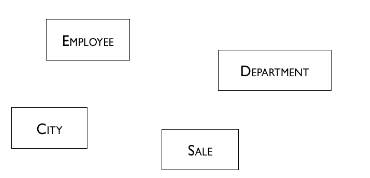
\includegraphics{2022-12-13-19-59-13.png}


\subsubsection{Relationships Sets}

\hspace{.5cm} A relationship set represents an association between $2+$ entity sets. It is represented with a diamond with lines connected to the entity sets it is directly associated with. The diamond is similar to the entity set as it includes the name of the relationship inside the diamond:

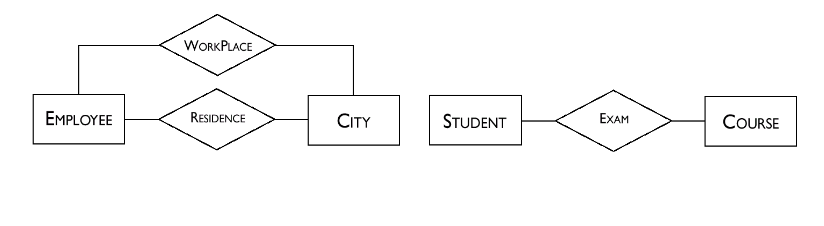
\includegraphics[scale=.7]{2022-12-13-20-09-52.png}

\subsubsection{Attributes}

\hspace{.5cm} Attributes describe the elementary properties of the elements of a model. These are notated with a line protruding from an entity, with a small circle labelling the attribute:

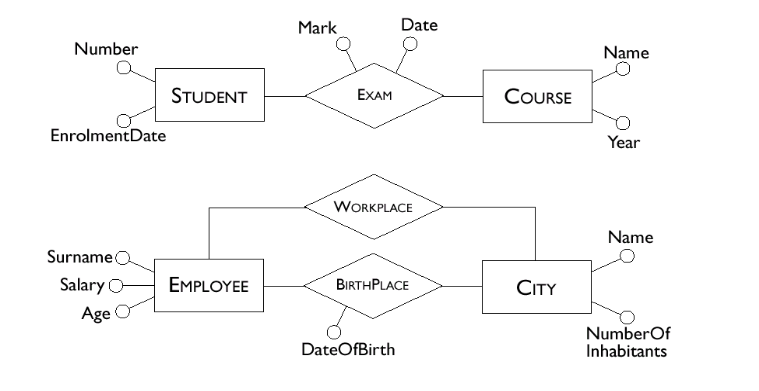
\includegraphics[scale=.7]{2022-12-13-20-16-19.png}

\subsubsection{Composite Attributes}

\hspace{.5cm} Composite Attributes are just groupings of similar attributes to improve clarity:

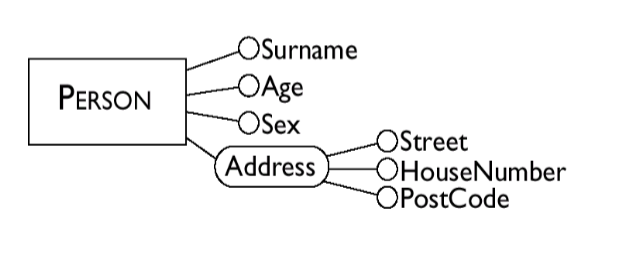
\includegraphics[scale=.7]{2022-12-13-20-17-36.png}

\subsubsection{Keys}

\hspace{.5cm} Keys are denoted in entities by filled in circles, in the case of a one attribute key, or a line with a ``knob'':

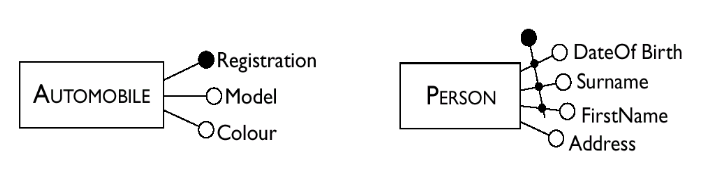
\includegraphics[scale=.7]{2022-12-13-20-19-34.png}




\begin{note}
    The graphics from this chapter are taken from the \textbf{ER-part1} slides, created by Manos Papagelis, Ryan Johnson, John Mylopoulos, 
    Arnold Rosenbloom, Renee Miller and Diane Horton.
\end{note}


\section{Cardinalities of Entity Relationships}

Cardinalities allow us to further describe how a relationship interacts with the entities it is connected to. Sometimes it is important to describe that there should be a certain amount, or range, of relationships for each tuple in an entity. These cardinalities are represented with a tuple, $(min, max)$, where the left hand side indicates the minimum number of relationships for a tuple, and the right indicates the maximum. We include this tuple on the line directly leaving the entity whose tuples' number of relationships we are describing:

\begin{center}
    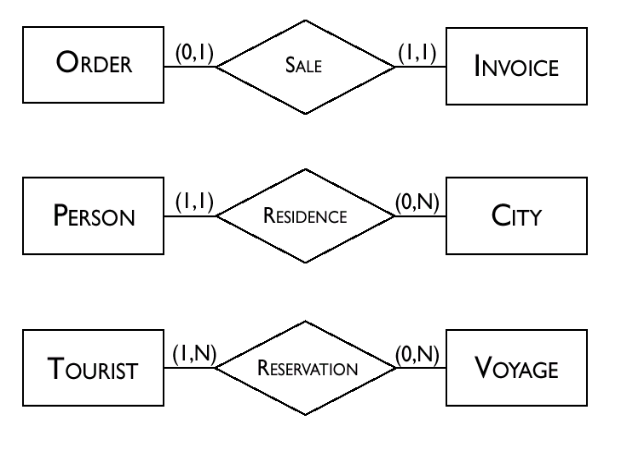
\includegraphics[scale = .75]{2022-12-13-20-30-47.png}
\end{center}

The cardinality can be interpreted with the following:\\
For minimum cardinality: (\textbf{min}, max):
\begin{enumerate}
    \item $0$: tuples in this entity do not need a relationship, the relationship is \textbf{optional}
    \item $\geq1$: tuples must have at least the minimum number of relationships, the relationship is \textbf{mandatory}
\end{enumerate}
For maximum cardinality: (min, \textbf{max}):
\begin{enumerate}
    \item $0$: this makes no sense
    \item $1$: tuples must have at most one relationship, meaning all relationships are \textbf{unique}
    \item $>1$: tuples may have up to the maximum number of relationships, and hence can be associated with \textbf{multiple} instances
    \item $N$: tuples have no upper limit of relationships
\end{enumerate}

\vspace{.5cm}
 
\dfn{Multiplicity of Relationships}{
    The multiplicity of a relationship describes the maximum number of relationships for each entity. Let $E_1$ and $E_2$ be two entities participating in a relationship $R$ with cardinalities $(n_1, N_1)$ and $(n_2, N_2)$ respectively. \\
    The multiplicity of $R$ is defined as $N_1$-to-$N_2$ or $N_2$-to-$N_1$ equivalently. 
}
\vspace{.5cm}
 

\begin{note}
    Cardinalities can also be used to describe the number of instances of a specific attribute. This has been omitted as it is usually an indication of a model which needs another relationship and entity to describe the multiplicity of said attribute. 
\end{note}


\section{Keys in Entity/Relationship Models}

As described in section in the earlier section on the basic elements on an Entity/Relationship Model, keys are represented in models with a filled circle or line with a knob. Where all attributes pierced by the line are a part of the key for the entity. In most cases, keys are unique to the entity and considered internal keys:

\begin{center}
    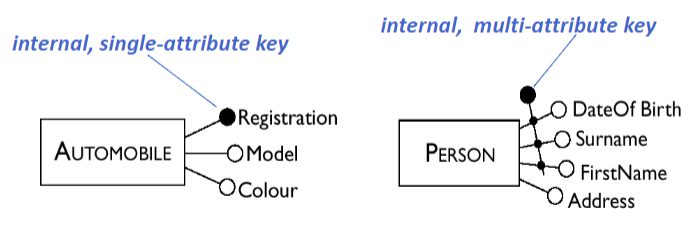
\includegraphics[scale=.85]{2022-12-13-20-57-04.png}
\end{center}

In some cases, keys are not strictly internal. This occurs when another entity sets do not have a key and must depend on another entities keys. To indicate this there is a line from the previous key extending to the line between the relationship and entity:

\begin{center}
    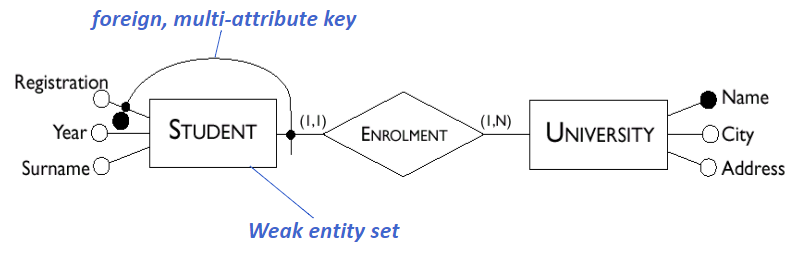
\includegraphics[scale=.8]{2022-12-13-21-00-54.png}
\end{center}

\dfn{Weak Entity Set}{
    An entity set is defined as weak when there is an entity who does not have a key among its own attributes. This means it depends on another entities or relationships key, requiring a foreign key. 
}

\subsubsection{Keys For Relationship Sets}
Often the key for a relationship is not explicit and is instead inferred from the entities it is connected to. This means its key is the union of all the entity's it is connected to's keys. The following example describes this:

\begin{center}
    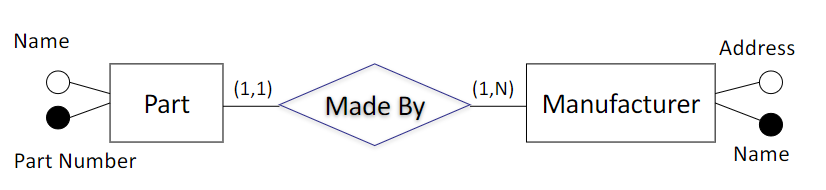
\includegraphics[scale=.7]{2022-12-13-21-18-41.png}
\end{center}

\ex{}{
    The Entity/Relationship Model above describes the parts made by a manufacturer. Since each entity has a key, we infer the key of the \textbf{Made By} relationship as the keys of the entities it connects: \underline{Part Number} and \underline{Name}
}
For a foreign key of an entity to come through a relationship, that entity must have a $(1,1)$ cardinality with the relationship. Otherwise we introduce the key being violated as when more the maximum is greater than one, the key could be duplicated, and when the minimum is less than one, the key can be \textbf{NULL}, both of which are contradictions of it being a key. A foreign key can also reference a key of an entity that is of itself a foreign. The one caveat is there must not be loops. Therefore, there must be at least one internal key in an E/R.


\section{From E/R Model to Database Schema}

The obvious next step after creating an Entity/Relationship model that one is happy with is to create a database schema from it. Before converting a model to a schema it is important to ensure that the model is in the correct preferred structure for a schema. If it is not we can restructure it as follows:

\begin{enumerate}
    \item \textbf{Remove Redundancy} This usually takes form in attributes that reference the same data, across entities. These attributes should be inferrable through relationships. It is also important to not induce redundancy by squashing too many relationships into one entity. This creates redundancy we described in the design theory chapter.
    \item \textbf{Entity Sets or Attributes?} Sometimes the question is wether to represent data as a separate attribute or as an entity. In some cases the decision is obvious, such as when there is a relationship between two entities where the cardinality of both sides is $(1,1)$ and one of the entities has only one attribute. In this case it is obviously favorable to combine the entities as there will be no redundant information. In cases of $N$-to-$N$ it could create too much functional redundancy by combining the entities. Other cases it is less clear. A good rule of thumb is to only consider squashing entities who's relationship is $1$-to-$something$ and  are more applicable as \textit{details} of another entity than as a unique \textit{thing}. 
    \item \textbf{Limit Weak Entity Sets} This improves clarity of the model. This can usually done by assigning IDs to entities without a key, but is not always possible:
    \ex{}{
        Given two entities \textbf{University} and \textbf{Student} with an \textbf{Enrolled} relationship. Unfortunately there is no unique identifier for students as student numbers between universities could be the same for two different students. Unfortunately, it is unlikely that there could be an 
        agreement to assign unique student numbers 
        across all students in the world. This is a case where foreign keys are required.
    }
    \item \textbf{Ensuring Keys Are Applicable to Schemas} This means that we must ensure that keys are applicable to schemas. Obviously this means any attributes that may be part of keys can not become or assume \textbf{NULL} values. Then there are other preferable qualities such as ensuring that keys have the minimum number of attributes and integers.
    \item \textbf{Removing Attributes with Cardinality > 1} It is not possible to have a container type for attributes. This means that any attribute that has been indicated as being able to support multiple entries, should be turned into a single entity.
\end{enumerate}







\end{document}


